\section{Infrastructure}
\label{sec:fdsp-tc-infr}


%%%%%%%%%%%%%%%%%%%%%%%%%%%%
\subsection{Introduction}
\label{sec:fdsp-tc-infr-intro}

The infrastructure needed to install the \dword{fd} includes the DSS, the electronics mezzanine on the cryostat roof (including racks), cable trays, the underground cleanroom with related installation equipment, piping inside the cryostat, and the coldboxes. 
 The major infrastructure provided by the installation group is described below. 
 Separate sub-sections are included for the DSS, the Cryostat roof infrastructure, Cryostat internal infrastructure, Cleanroom, and Cryogenics and cold-boxes.

In addition to the equipment described below many smaller items will be needed like: a small machine shop, scissor lifts, rigging equipment, hand tools, diagnostic equipment (including oscilloscopes, network analyzers, and leak detectors), local storage with some critical supplies and personal protective equipment (PPE).  

%%%%%%%%%%%%%%%%%%%%%%%%%%%%
%\subsection{Detector Support System}
\subsection{Detector Support System}
\label{sec:fdsp-tc-infr-dss}

The \dword{dss} provides the structural support for the \dword{spmod} inside the cryostat.  
It also provides the necessary infrastructure to move the detector elements into place during
assembly. 
The \dword{dss} is a new design, quite different from the \dword{pdsp} \dword{dss}. It is described in some detail in this
section. 
The detector elements supported by the \dword{dss} include the \dwords{ewfc}, the \dwords{apa}, and the \dwords{cpa} with top and bottom \dword{fc} panels. The nominal load of the detector elements both dry (in air) and wet (under \dword{lar}) are shown in Table \ref{tab:installation-DSS-load}. The weights listed are the current design weights and do not include any margin for future design changes.  
The \dword{dss}, however, is designed so the weights can be doubled, and it would still meet the requirements of the design codes.  
Deformations would increase due to any increase in loads, and this effect should be evaluated.
\begin{comment}
\begin{dunetable}
[DSS Loads]
{l|c|cc|cc}
{tab:installation-DSS-load}
{The expected dry and wet stratic loads for the DSS.}
\multicolumn{2}{c}{} &  \multicolumn{4}{|c}{Dry Weight}\\ \toprowrule
\multicolumn{2}{c|}{} & \multicolumn{2}{c|}{Unit Weight} & \multicolumn{2}{c|}{Total Weight}  \\ \colhline

Detector Component &\# Units& (kg)&(lbs) & (kg) &(lbs)\\ \colhline
Detector Support Structure (DSS) (not in liquid) & 1 &NA&NA& 12318  & 27100 \\ 
\colhline
Anode Plane Assembly (Installed APA pair/No cables)& 75&1184 &2604 &88768  &195290\\ 
\colhline
Cathode Plane Assembly (CPA) & 100& 233 & 513 & 23331 & 51327 \\ 
\colhline
Top or Bottom Field Cage module (FC TB)& 400&149 & 328	 & 59679 & 131294\\ 
\colhline
CE Cables &750& 182 & 400 & 13636 & 30000\\
\colhline
Field Cage Endwall  & 8	&904 &	1989  & 7234 & 15914\\ 
\colhline
{\bf Total} &  & & & 204966 &	450925\\ 
\colhline
\toprowrule

\multicolumn{2}{c|}{} &  \multicolumn{4}{c}{Wet Weight}\\
\toprowrule
Detector Support Structure (DSS) (not in liquid) & 1 & NA & NA & 12318 & 27100 \\ 
\colhline
Anode Plane Assembly (Installed APA pair/No cables)&75& &0 & 0 &0\\ 
\colhline
Cathode Plane Assembly (CPA) & 100& 45 & 99 & 4520 & 9943 \\ 
\colhline
Top or Bottom Field Cage module (FC TB)& 400 & 68 & 150	& 27359 & 60191 \\ 
\colhline
CE Cables & 75 & & & 13636& 30000 \\
\colhline
Field Cage Endwall & 8 & 283& 	622& 2263 & 4978\\  
\colhline
{\bf Total} &  & & &60096	 &132211 \\ 
\colhline
\end{dunetable}
\end{comment}

\begin{dunefigure}[\threed model of the \dword{dss} ]{fig:DSS}
  {\threed model of the \dword{dss} showing the entire
  structure on the left along with one \dword{apa} row and one
  \dword{cpa}-\dword{fc} row at each end. The right panel is a zoomed image
  showing the connections between the vertical supports and the
  horizontal I-beams.}
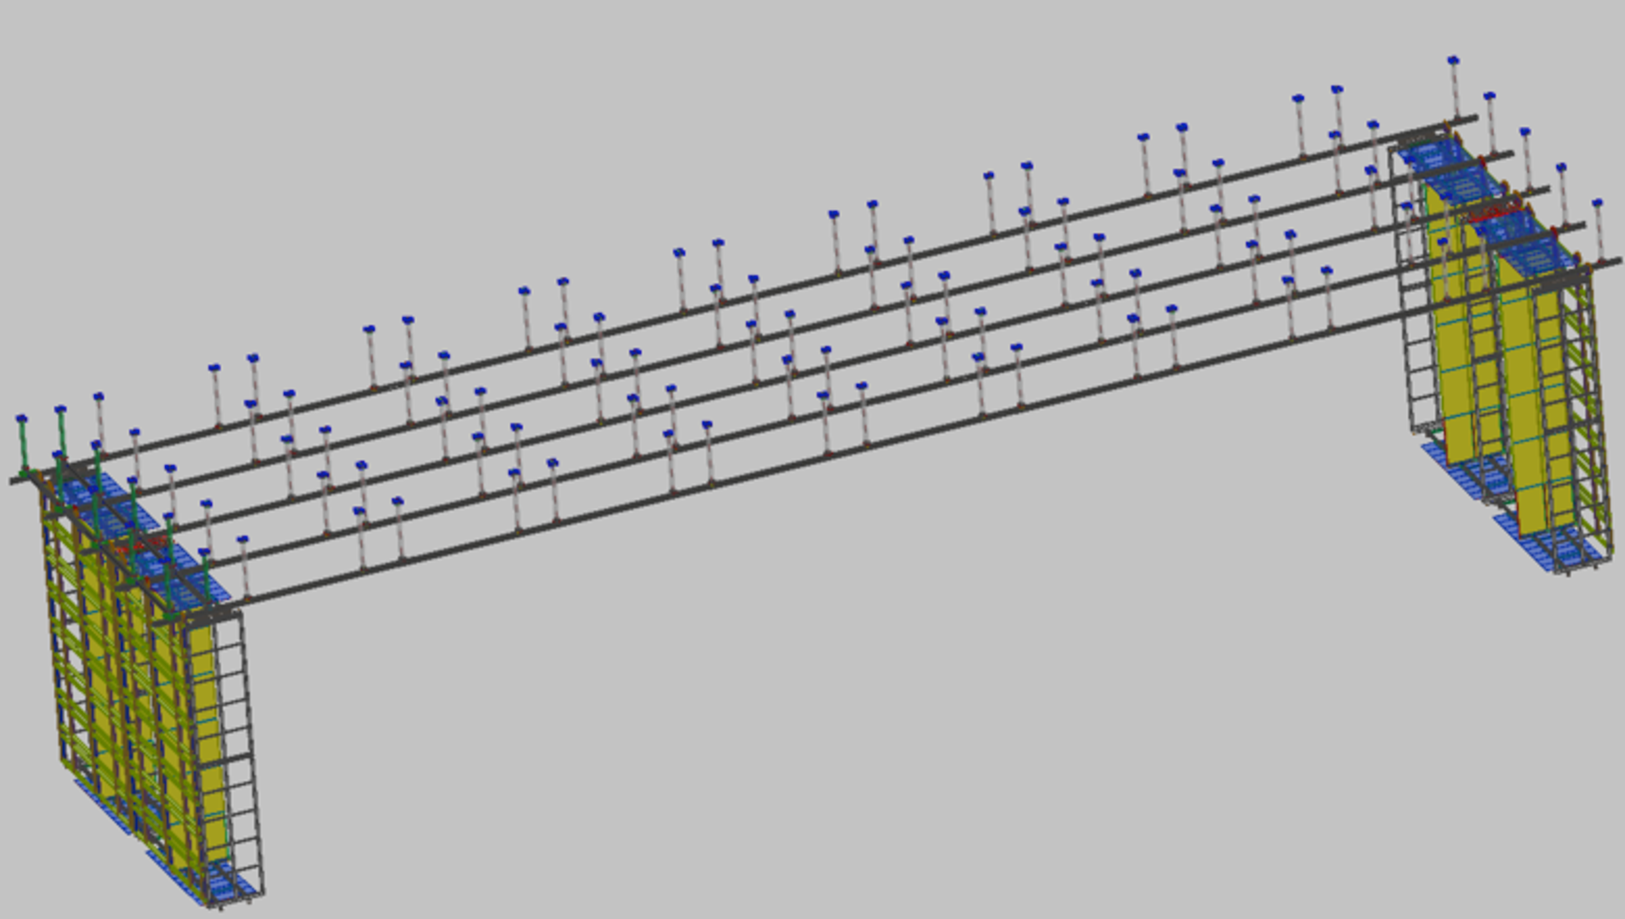
\includegraphics[width=.49\textwidth]{DSS-1.pdf}
 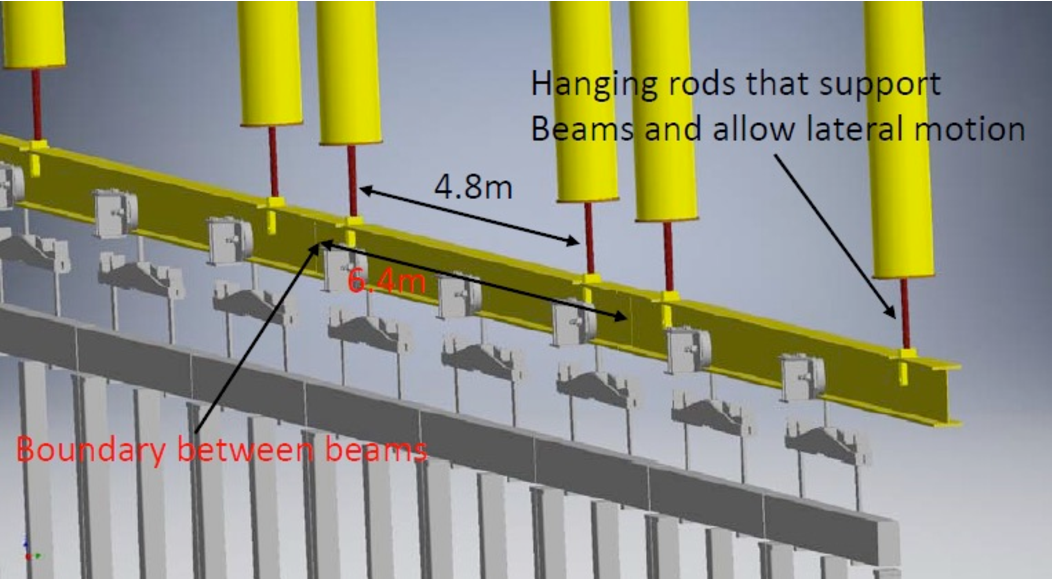
\includegraphics[width=.49\textwidth]{DSS-2.pdf}
\end{dunefigure}

The \dword{dss} is supported by the
cryostat outer steel structure through a series of \fdth{}s that cross through the cryostat insulation and anchored with flanges on
the cryostat roof. 
Inside the cryostat, a series of stainless steel I-beams are connected to the \fdth{}s and used to support the
detector. 
The \dword{dss} defines the location of the detector inside the cryostat and also defines how the detector elements move and contract as the detector is brought to \dword{lar} temperature. 
The design of the \dword{dss} encompasses the overall
structural design of the \dword{detmodule} because only after the elements are mounted to the \dword{dss} and connected do they make a unified mechanical structure. 
Figure~\ref{fig:DSS} (left) shows the \dword{dss} structure; there are
five rows of supports for the alternating rows of
\dword{apa}-\dword{cpa}-\dword{apa}-\dword{cpa}-\dword{apa}.  
The \dword{dss} is connected to the cryostat warm structure at a flange mounted on the outside of the cryostat.  
Figure~\ref{fig:DSS} (right)
shows the layout of these structural \fdth{}s.

The \dword{dss} is designed to meet the following  requirements:
\begin{itemize}
 \setlength\itemsep{1mm}
\setlength{\parsep}{1mm}
\setlength{\itemsep}{-5mm}
% \small
\item Support the weight of the detector;
\item Accommodate cryostat roof movement during filling, testing, and operation;
\item Accommodate variation in \fdth locations and
  variation in the flange angles due to installation tolerances and
  loading on the warm structure;
\item Accommodate shrinkage of the detector and \dword{dss} from ambient
  temperature to \dword{lar} temperature;
\item Define the positions of the detector components relative to each other; 
\item Provide electrical connection to the cryostat ground and remain electrically isolated from the detector;
\item Allow support penetrations to be purged with gaseous argon to prevent contaminants from diffusing back into the liquid; 
\item Ensure that the instrumentation cabling does not interfere with the \dword{dss};
\item Consist entirely of components that can  
be installed through the \dword{tco};
\item %Design to m
Meet AISC-360 or appropriate codes required at \dword{surf};
\item %Design to m
Meet seismic requirements one mile underground at \dword{surf};
\item Consist entirely of %All materials must be 
materials compatible for operation in ultrapure \dword{lar};
\item Ensure that beams are completely submerged in \dword{lar};
\item Ensure that detector components are not less than \SI{400}{mm} from the membrane flat surface;
\item Ensure that the supports do not interfere with the cryostat I-beam structures;
\item Ensure %Design such 
that the detector's lower \dword{gp} is lies over the cryogenic piping and that the tops of the \dword{dss} beams are submerged in \dword{lar} while leaving a \SI{4}{\%} ullage at the top of the cryostat;
\item Include the infrastructure necessary to move the \dword{apa} and
  \dword{cpa}-\dword{fc} assemblies from outside the cryostat through the
  \dword{tco} and to the correct position.
\end{itemize}

  The \dword{dss}
consists of pairs of \fdth{}s that support \SI{6.4}{m}-long
W10x26 stainless steel I-beam sections. The proposed design of the
\dword{dss} has \num{10} I-beam segments per row for a total of
\num{50} I-beam segments. Each I-beam is suspended on both ends by
rods from \fdth{}s that penetrate the cryostat roof.  %In the cold condition
When cold, each I-beam shrinks, causing gaps to form between
\dword{apa}s that are adjacent but supported on separate beams.
\dword{apa}s that are supported on the same beam will not have gaps
develop because both the beam and \dword{apa}s are stainless steel so
they shrink together.  Each beam is supported by a nearly
\SI{2}{m} long rod that allows the beam support to move as the beam
contracts.


The feedthrough consists of a flange and $6 ^{''}$ OD structural tube welded to it that extends through the cryostat insulation.  
There is a
nominal \SI{10}{mm} gap between the OD of the tube and the ID of the clearance tube in the cryostat. \fixme{OD and ID are not defined in the common glossary.}
The $6 ^{''}$ tube provides lateral support to the I-beams during installation.
Running down the center of the feedthrough is a $1^{"}$ diameter rod supported at a swivel washer at the flange and then supported by the
I-beam at a clevis.  The gas seal is obtained by Conflat Flange and a
bellows that seals around the swivel washer.  The lateral position and height of the rod can be adjusted $\pm$1 inch to accommodate tolerances in positioning cryostat crossing tubes. Figure \ref{fig:DSS-lateral-support} shows the end of the $6 ^{''}$ tube and how it locks the I-Beam into position. 

\begin{dunefigure}[DSS support for lateral loads ]{fig:DSS-lateral-support}
  {Left panel shows how the central support rod is locked in postion during detector installation. The outer $6 ^{''}$ tube is used to fix the support clevis in position. The right panel shows the system as it is connected to the I-Beam.}
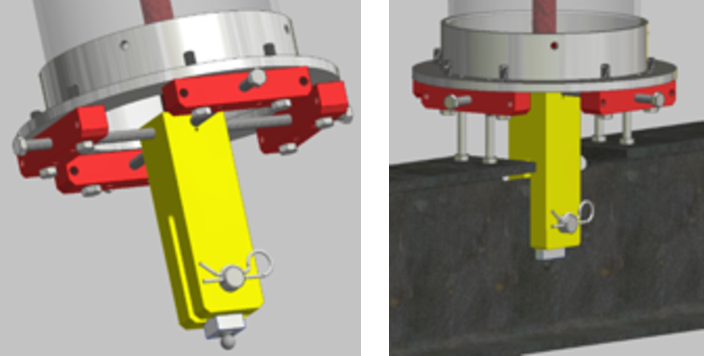
\includegraphics[width=.75\textwidth]{graphics/dss-lateral-support.pdf}
\end{dunefigure}

After the detector has been installed all restraints will be released to allow motion as the detector contracts during cool down.  The two hangars that support each \dword{dss} beam will contract and move toward each other by 13.1 mm along the axis of the detector.  
The drift distance will shrink by 7.4mm caused by the contraction of the field cages.  The detector is symmetric in the drift direction around the center \dword{apa}.  The drifts on either side of the center \dword{apa} will  shrink toward the center while the center \dword{apa} remains unmoved.  This results in the \dwords{cpa} moving 7.4mm toward the center and the outer \dword{apa}s moving 14.8mm (2*7.4mm) toward the center.  The hanging rod is designed to have a range of motion of 15mm in the drift direction to accommodate this shrinkage.




Detector components are installed using a shuttle beam system as
illustrated in Figure~\ref{fig:shuttle}.  
The last two columns of
\fdth{}s (eastern-most) support temporary beams that run
north-south, perpendicular to the main \dword{dss} beams.  
A shuttle beam has trolleys mounted to it and transverses 
north-south until it aligns with the required row of \dword{dss} beams.  
The last \dword{apa} or \dword{cpa} in a row is supported by the shuttle beam, which is bolted directly to the \fdth{}s once it is in place.  
As the last \dword{cpa} or \dword{apa} in each row is installed, the north-south beams are removed.

\begin{dunefigure}[\threed models of the shuttle beam end of the \dword{dss}]{fig:shuttle}
  {\threed models of the shuttle beam end of the \dword{dss}. The figures show how an \dword{apa}
is translated into position using the north-south beams until it lines up with the correct
row of I-beams.}
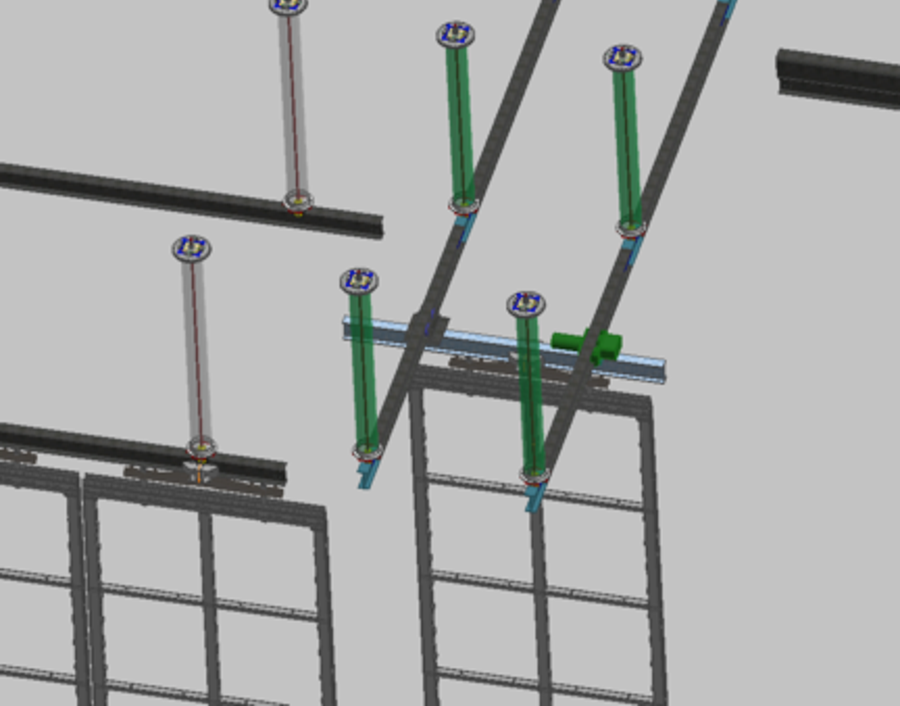
\includegraphics[width=.49\textwidth]{/Shuttle-1.pdf}
 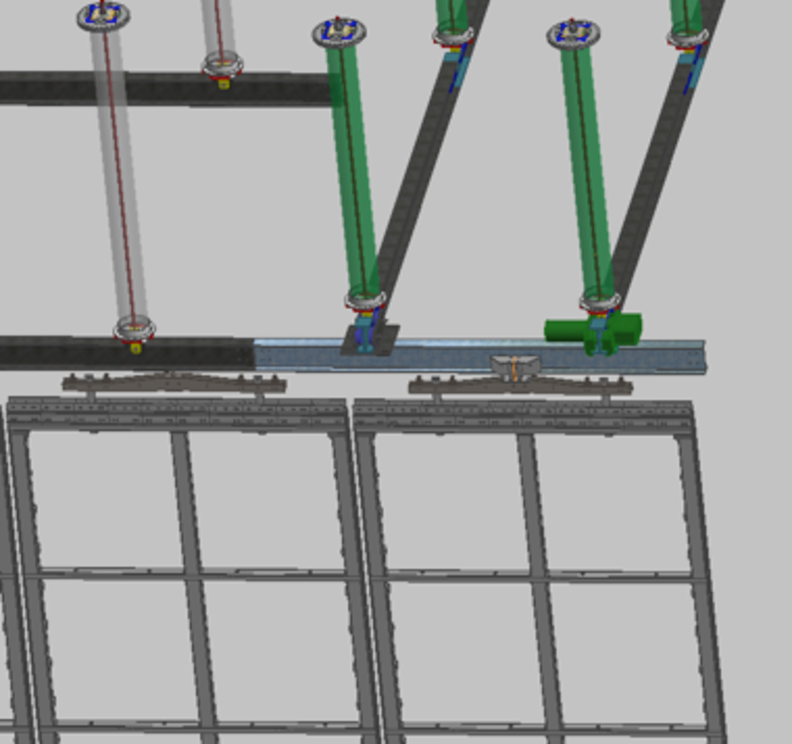
\includegraphics[width=.42\textwidth]{shuttle-2.pdf}
\end{dunefigure}

A mechanical interlock system  prevents trolleys
from passing the end of the shuttle beam unless it is aligned with a
corresponding \dword{dss} beam.  The shuttle beam and each detector component are
moved using a motorized trolley.  A commercially available motorized
trolley will be modified as needed for the
installation. 




\begin{dunefigure}[Prototype of the motorized DSS trolley ]{fig:DSS-trolley}
  {Prototype of the motorized DSS trolley that will push the APA and CPA along the I-beams and through the switchyard.}
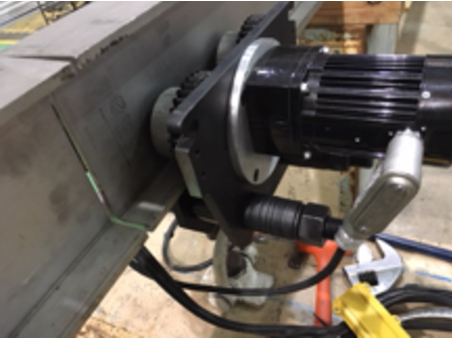
\includegraphics[width=.49\textwidth]{graphics/DSS-trolley.pdf}
\end{dunefigure}



A mock-up of the shuttle system will be constructed to test the
mechanical interlock and drive systems for the shuttle beam
for each \dword{detmodule}.  Tests will be conducted to evaluate the level of
misalignment between beams that can be tolerated and the amount of
positional control that can be achieved with the motorized trolley. We plan to construct a full scale prototype of a section of the  switchyard and perform tests at floor level. Later, the test program will be expanded at Ash River, where a full scale installation test will be performed. This is described in the installation \dword{qa} section.


%%%%%%%%%%%%%%%%%%%%%%%%%%%%
\subsection{Cryostat Roof Infrastructure}
\label{sec:fdsp-tc-infr-cryo-roof}



\begin{dunefigure}[Mezzanine and electronics racks]{fig:mezzanine}
  {The electronics racks sitting on the DUNE electronics mezzanine is shown. The top image is a view from above the detector looking at the racks from the side. In this view the cavern and cryogenics mezzanine are hidden. The bottom view is from the end of the cryostat looking over the roof. Here the access stairs to the mezzanine are shown.}
 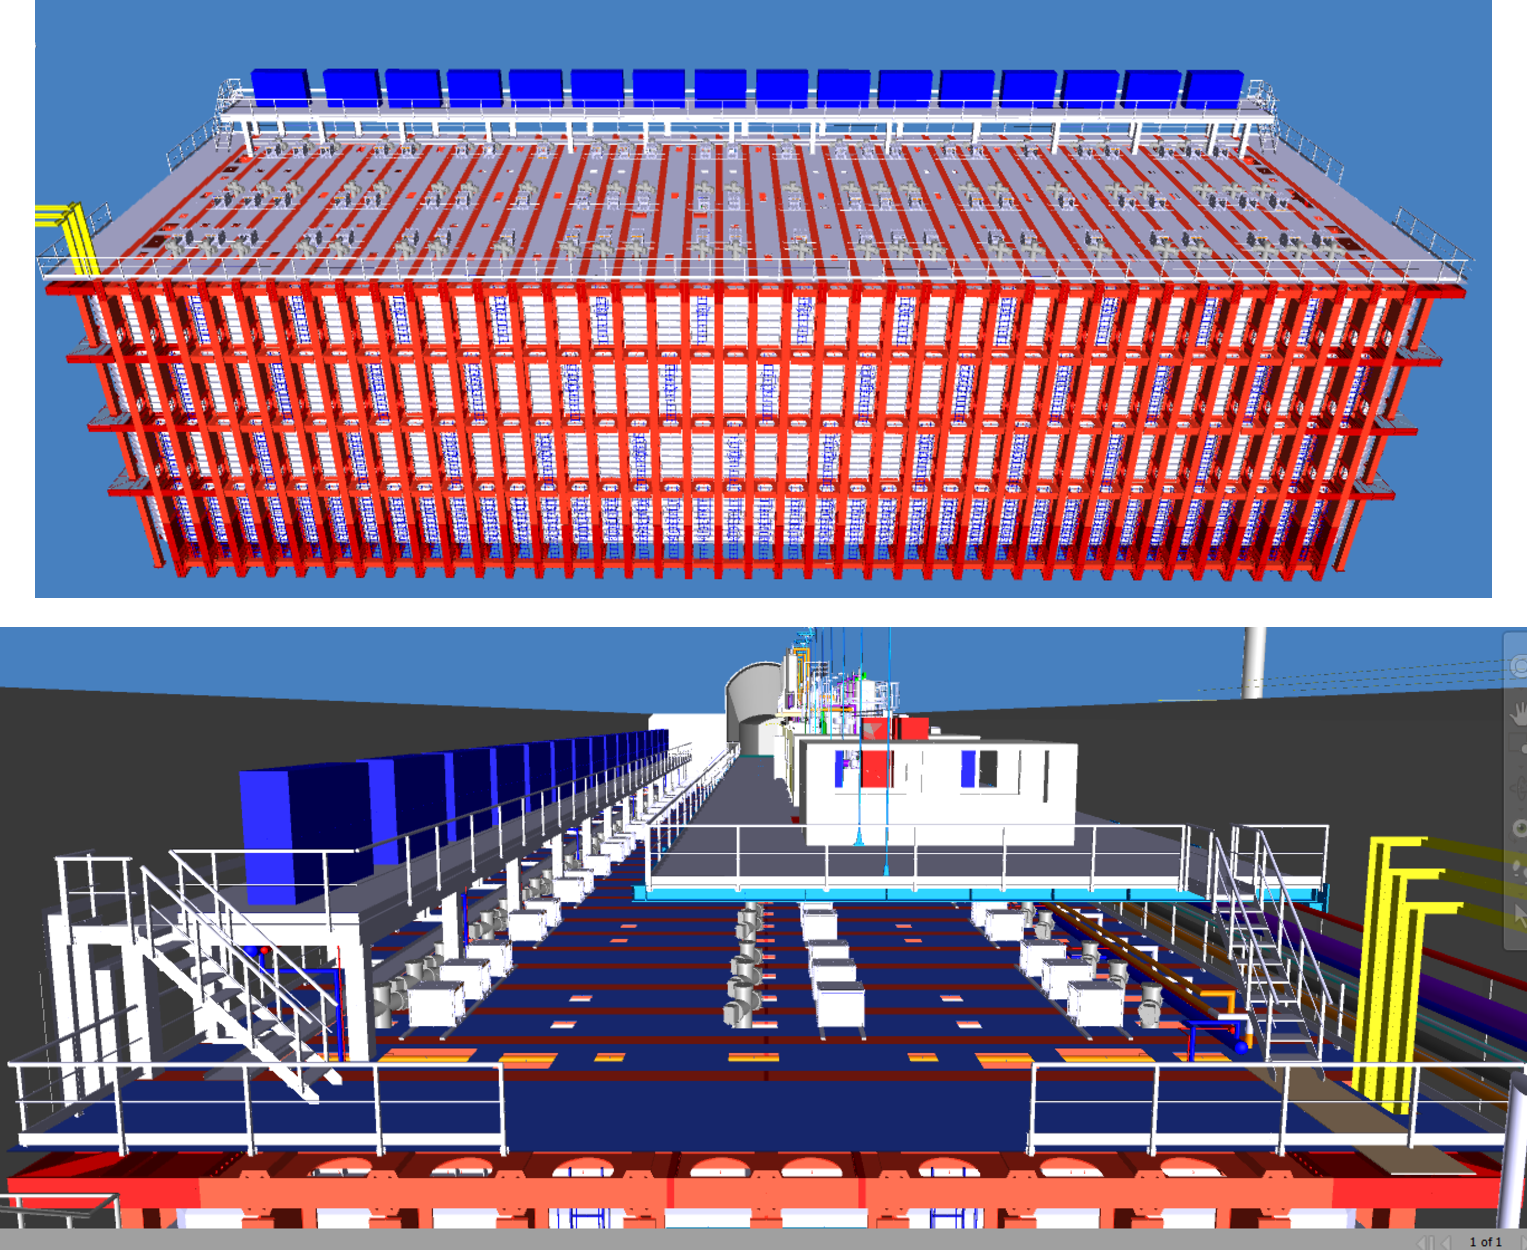
\includegraphics[width=\textwidth]{mezzanine.pdf}
\end{dunefigure}

\begin{dunefigure}[Electronics rack contents]{fig:rack-build1}
  {The nominal contents of the electronics racks on the mezzanine is shown. Each rack is configured to consume less than 3.5 \si{kW}. }
 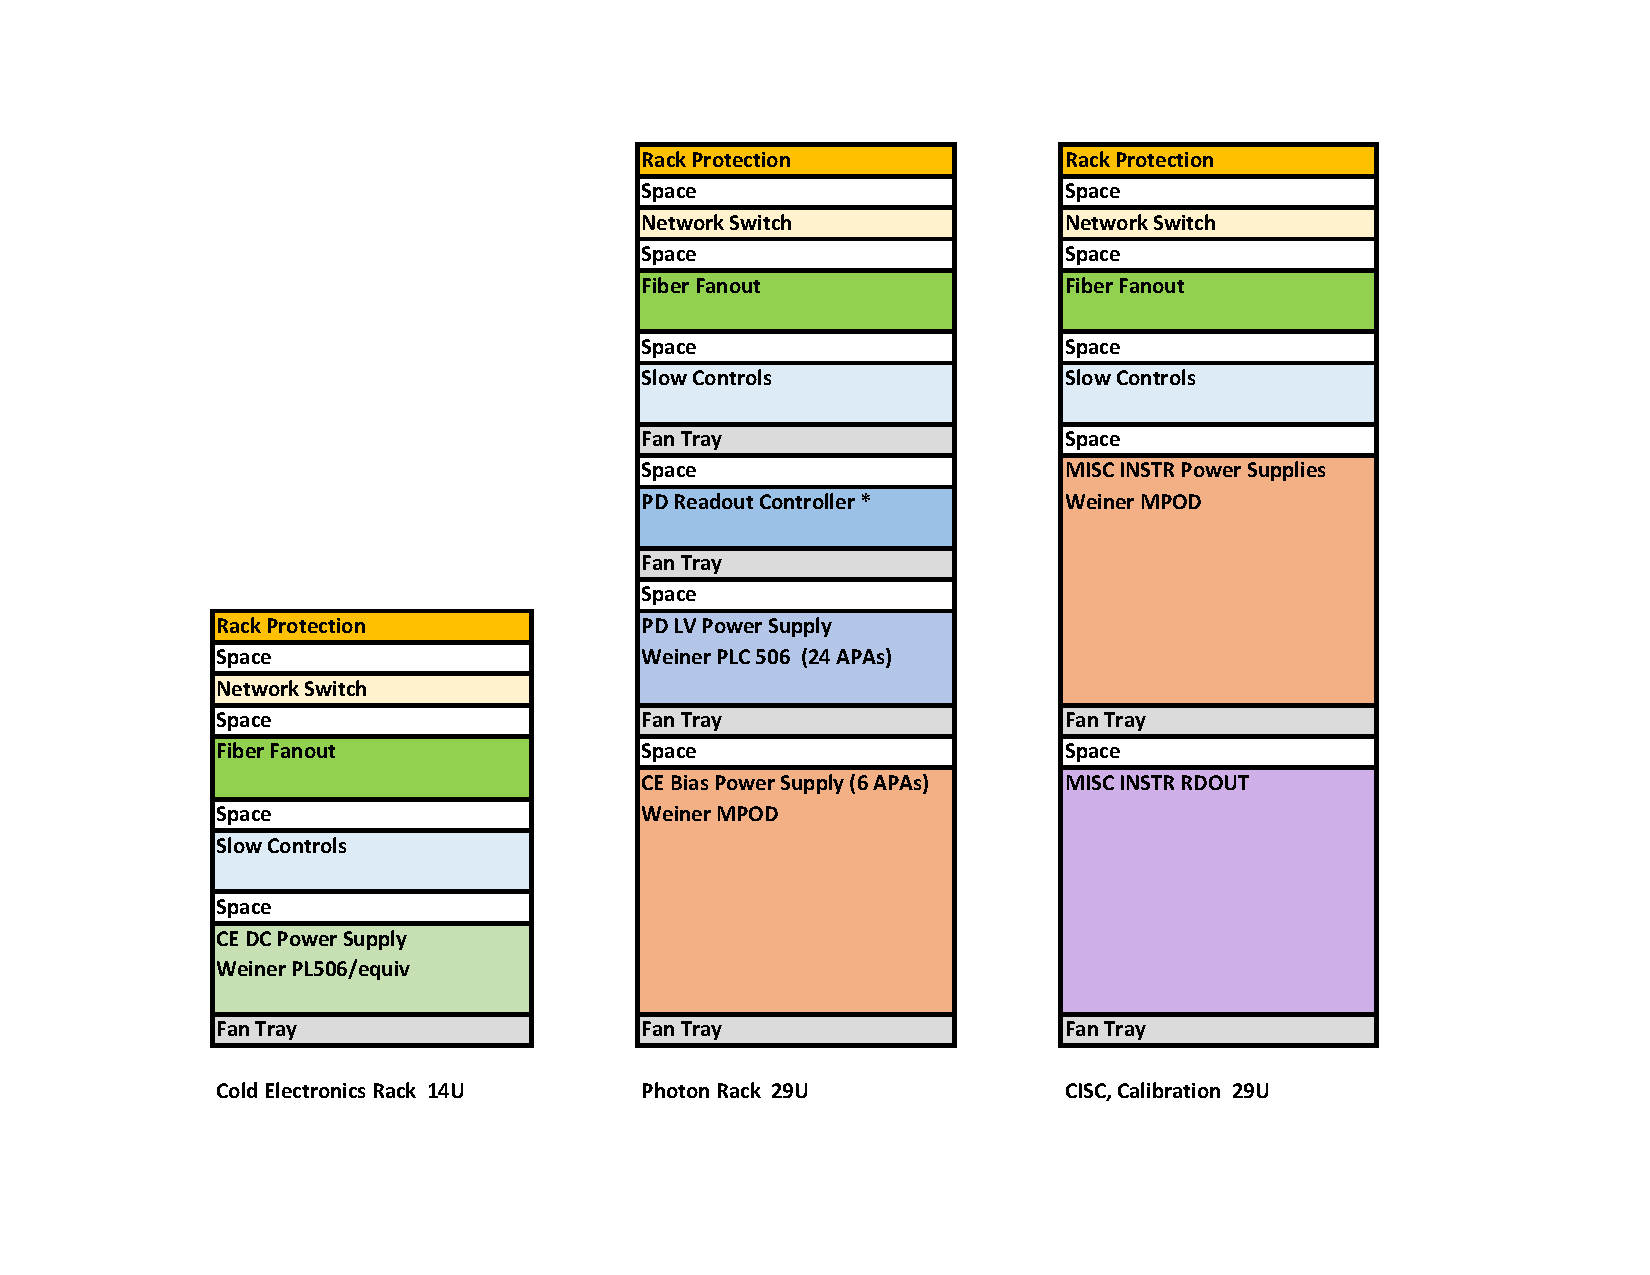
\includegraphics[width=.98\textwidth]{graphics/rack-build1.pdf}
\end{dunefigure}

The top image in Figure \ref{fig:mezzanine} shows the DUNE electronics mezzanine with the 42U racks placed on top. 
During the initial design steps it became clear that the constraints placed on the rack location by the many DSS support feedthrus, the electronics feedthru and the I-beams themselves make distributing the racks on the roof very challenging. 
By constructing a fixed mezzanine above the cryostat at the same height as the cryogenic mezzanine the electronics feedthrus are kept clear. 
This configuration also makes working on the electronics much easier as there are no local obstacles and all the racks are in one place.
The racks are on detector ground so the mezzanine is also on detector ground so it can simply be bolted to the cryostat I-beams. 
As seen in Figure \ref{fig:mezzanine} there are 16 groups of 5 racks on the mezzanine for a total of 80 racks. 
The heat load inside the detector racks is expected to be dissapated through air flow generated by cooling fans.  The major heat load resides with the cold electronics and photon electronics located near the cryostat feedthroughs.  If rack mounted fans do not provide sufficient cooling,  CF will provide sufficient water cooling capacity at the entrance to the North cavern to accommodate the maximum heat load. 
Twenty-five racks will be needed for the cold electronics low voltage power and twenty-five racks are available for APA wire bias voltage, the photon detector power and miscellaneous. 
The remaining 25 racks will be available for slow control, calibration and miscellaneous other equipment. 
Small racks will also be placed near the electronics feedthrus for the PD readout electronics and optical patch panels. 
If this is not adequate then additional racks can be placed on the cryostat roof. 
The present rack build for this layout is shown in figure \ref{fig:rack-build1}. The modules inside the racks are distributed to keep the power consumption for each rack below 3.5 \si{kW}.
The racks to be installed will be 42U high so significant extra capacity is foreseen though if added electronics is needed for the cold electronics it would be necessary to install the modules in a PD rack to keep under the power limit per rack.
The 12U high mini-racks near the feedthru flanges will be relatively empty as the PD readout is only expected to need around 2U in height and the CE patch panel less than 1 U. The mini-racks are shown in the lower panel of Figure \ref{fig:rack-build1} as the gray rectangles near the electronics tees.
The north-south cable trays running from the electronics mezzanine to the electronics feedthru will be routed under the floor of the cryostat roof next to the cryostat I-beams. 
By doing this the roof can be kept reasonably clear so equipment can be transported across the cryosat roof as needed. 
The gap between the web of the I-beams is 1.2 \si{m} so a 200--300 \si{mm} wide cable tray can be installed while still leaving enough space to stand on the roof and work on the electronics crates. 
The cable trays between the CUC and the electronics mezzanine will run along the West end of the cryostat under the floor. 
It is estimated that only 1/2 of the 1.6 \si{m} space is needed so  the cable tray quantity could in principal be doubled if necessary. 

It is expected that flooring similar to the 25 \si{mm} thick plywood used at protoDUNE will be used for the final DUNE detector. 
The flooring material must be easy to cut as it needs to fit around numerous obstacles and pipes on the roof, it needs to be light enough to lift up if access below is needed, and it has to support the load of a person or small cart. 
It will be investigate what type fire retardant options exist in the US and input from the FNAL fire life-safety group will be solicited. 

The air filtration for the cleanroom and inside the cryostat will also be placed on the cryostat roof. The present plan is to place fan filter units near the manholes on the East end of the cryostat. Initial calculations indicate sufficient airflow is possible to support one air exchange per hour inside the cryostat. The detail design of the air handling system has yet to begin.


\begin{dunefigure}[Cryostat crossing tube design]{fig:crossingtube}
  {Draft drawing of the cryosat crossing tubes. The hatched region is the cryostat insulation.}
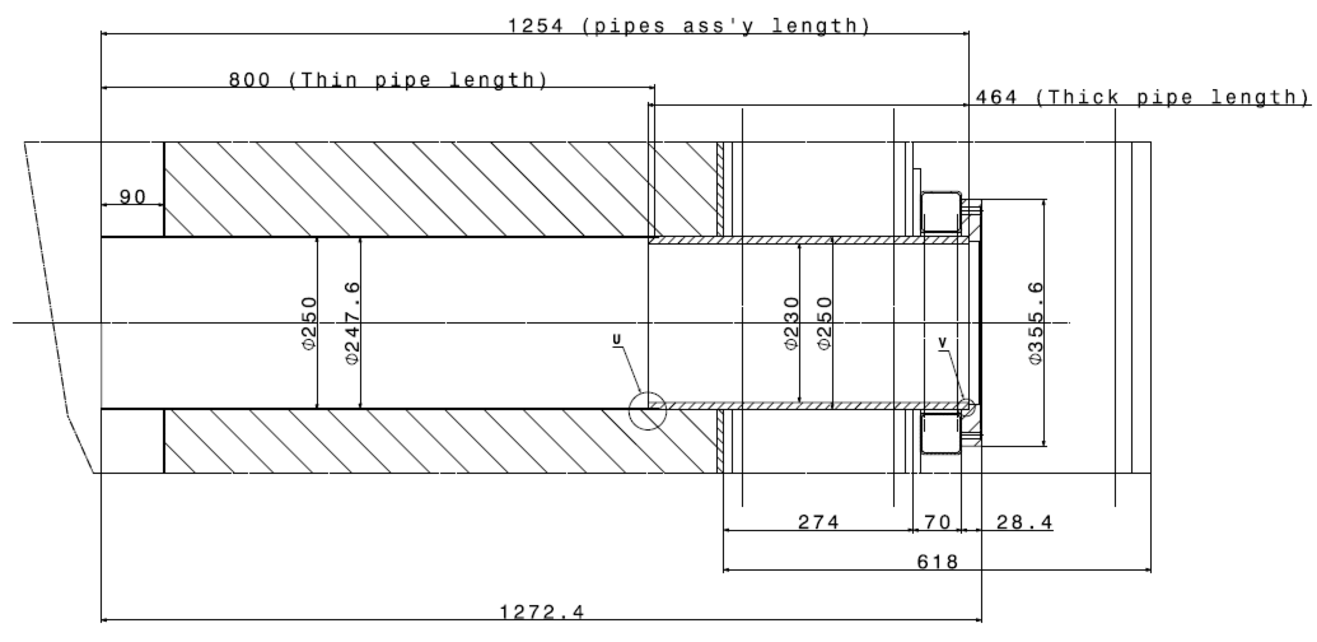
\includegraphics[width=.85\textwidth]{crossingtube}
\end{dunefigure}

One of the most critical components of the roof infrastructure are the cryostat crossing tubes. These are the vacuum components that penetrate the cryostat roof and connect to the cold cryostat membrane. The top flange of the crossing tube supports the electronics feedthru or the detector support flanges and must be directly tied to the steel I-beams for support. Accurately locating the crossing tubes and installing them true to vertical is important to ensure the interface to the cryostat membrane can be made. A draft assembly drawing of the crossing tube is shown in Figure \ref{fig:crossingtube}. The tube consists of a 464 \si{mm} long stainless steel pipe with 1 \si{cm} wall. The thin stainless steel tube that is welded to the cryostat membrane is welded to on end of the tube and custom CF flanges are welded to the other end. The \si{cm} thick tube is welded to the steel roof plates.


To ensure that the crossing tubes are adequately cleaned during the initial GAr purge and that air is removed from them, each crossing tube has a small side port connected to a network of pipes on the roof of the cryostat. During the initial GAr purge, argon gas is withdrawn from each port and analyzed to assess progress and determine when the system is ready to be cooled down. Due to the high number of crossing tubes, about 250 in the \dword{sp} configuration, the content from each port cannot be analyzed independently of all others. Five streams, each one collecting gas from about 50 crossing tubes are connected independently to the gas analyzers. Gas impurities accumulate in the ullage. During steady--state operations, GAr from the crossing tubes will be analyzed to ensure that the impurities are adequately removed from the GAr.    If additional cleaning of the ullage is required, the GAr withdrawn from all ports, or a smaller set of them, can be sent to the condenser, re--condensed and purified in the liquid phase along withe the rest of the \dword{lar}. In order to detect any possible leaks which could develop in the room temperature feedthrus over time simple O$^2$\ sensors monitor the return gas for traces of oxygen, which would be indicative of a leak.

Each detector has a power budget of 500 KVA. The total power budget available for use by detector electronics is derated to 400KW at the power distribution panels.  The cold electronics are the largest power load.  

The cold electronics dissipate 306 Watts per APA.  The low voltage power supplies have a controller which is about 35 Watts per APA and have an efficiency of approximately 85 percent.  This leads to approximately 400 Watts per APA, or a total load of 60 KW per detector.  The APA wire bias power supplies have a maximum load of 465 Watts per six APAs for a total budget of around 12 KW.  Some nominal amount of power will be used by cooling fans and heaters located near the feedthroughs, so the overall power budget for cold electronics should be below 75 KW.

The photon detector electronics which are based on the Mu2e electronics report a power load of approximately 6KW.  A power budget of 8KW should be used due to cable drops and  power supply inefficiencies.  It should be noted that these PD electronics are a significantly lower power load than the alternate ProtoDUNE solution of using SSP modules at a power load of approximately 72 KW per detector.

Each of the approximately 80 detector racks will have fan units, ethernet switches, rack protection and slow controls modules adding a load of about 500 Watts per rack, for a total of 40 KW.

A number of racks are reserved for cryo instrumentation.  The load of these 25 racks is conservatively estimated to be 2 KW per rack for a total of 50 KW.

Thus, an estimated 173 KW of power will be used by the detector.  If the photon detector finds it must go to a higher load SSP solution, a total of 237 KW is accounted for.  These numbers provide a safety factor of about two on our power estimates when compared to available power.


%%%%%%%%%%%%%%%%%%%%%%%%%%%%
\subsection{Cryostat Internal Infrastructure}
\label{sec:fdsp-tc-infr-cryo-int}

\fixme{Check text from David below!!}

%%%%Internal Cryogenics%%%%
\label{sec:fdsp-tc-internal-cryo}

The internal cryogenics comprises three sets of pipe distribution networks and two sets of sprayers. All pipes enter the cryostat from the top; some go all the way down to the floor, and others remain in the ceiling. On the floor are
\begin{itemize}
\setlength\itemsep{1mm}
\setlength{\parsep}{1mm}
\setlength{\itemsep}{-5mm}
\item \textbf{GAr distribution}: a set of pipes flowing GAr. These pipes are used only at the beginning to remove air that fills the cryostat. They have either a longitudinal slit or calibrated holes to distribute GAr uniformly along the length of the cryostat. Computational fluid dynamics simulations show that air will be removed from the system as long as GAr is flowing in at the right speed, calculated and experimentally verified as \SI{1.2}{m/hr}.


\item \textbf{\dword{lar} distribution}: two sets of pipes flowing \dword{lar}. These pipes are used to fill the cryostat and, during steady state operations, to return the \dword{lar} from the purification system. The pipes have calibrated holes to return the \dword{lar} uniformly throughout the length of the cryostat. This is very important for uniform purity. Four pumps circulate the \dword{lar}. Initially, all of pumps operate at once to achieve purity, but once the target purity is achieved, only one or two pumps remain in service. Two sets of pipes are needed to adequately distribute the \dword{lar} over this broad range of flow rates.
\end{itemize}

On the ceiling are

\begin{itemize}
\setlength\itemsep{1mm}
\setlength{\parsep}{1mm}
\setlength{\itemsep}{-5mm}
\item \textbf{Cool down sprayers}: Two sets of cool down sprayers are distributed along the long sides of each cryostat. One set distributes \dword{lar} using liquid sprayers that generate a conical profile of small droplets of liquid. The other set of sprayers distributes GAr to move the \dword{lar} droplets inside and cool down the detector and cryostat uniformly. These sprayers are being tested in \dword{pddp}. They are a variation of those implemented in \dword{pdsp}.
\end{itemize}

Figure~\ref{fig:internal-cryo-3D} shows the current layout of the internal cryogenics. 
%The current drawing of the internal cryogenics is presented in Figure~\ref{fig:internal-cryo-drawing}. 
The GAr pipes are in red, the \dword{lar} pipes in blue.

\begin{dunefigure}[Cryogenic piping inside the cryostat ]{fig:internal-cryo-3D}
  {Layout of the internal cryogenics.}
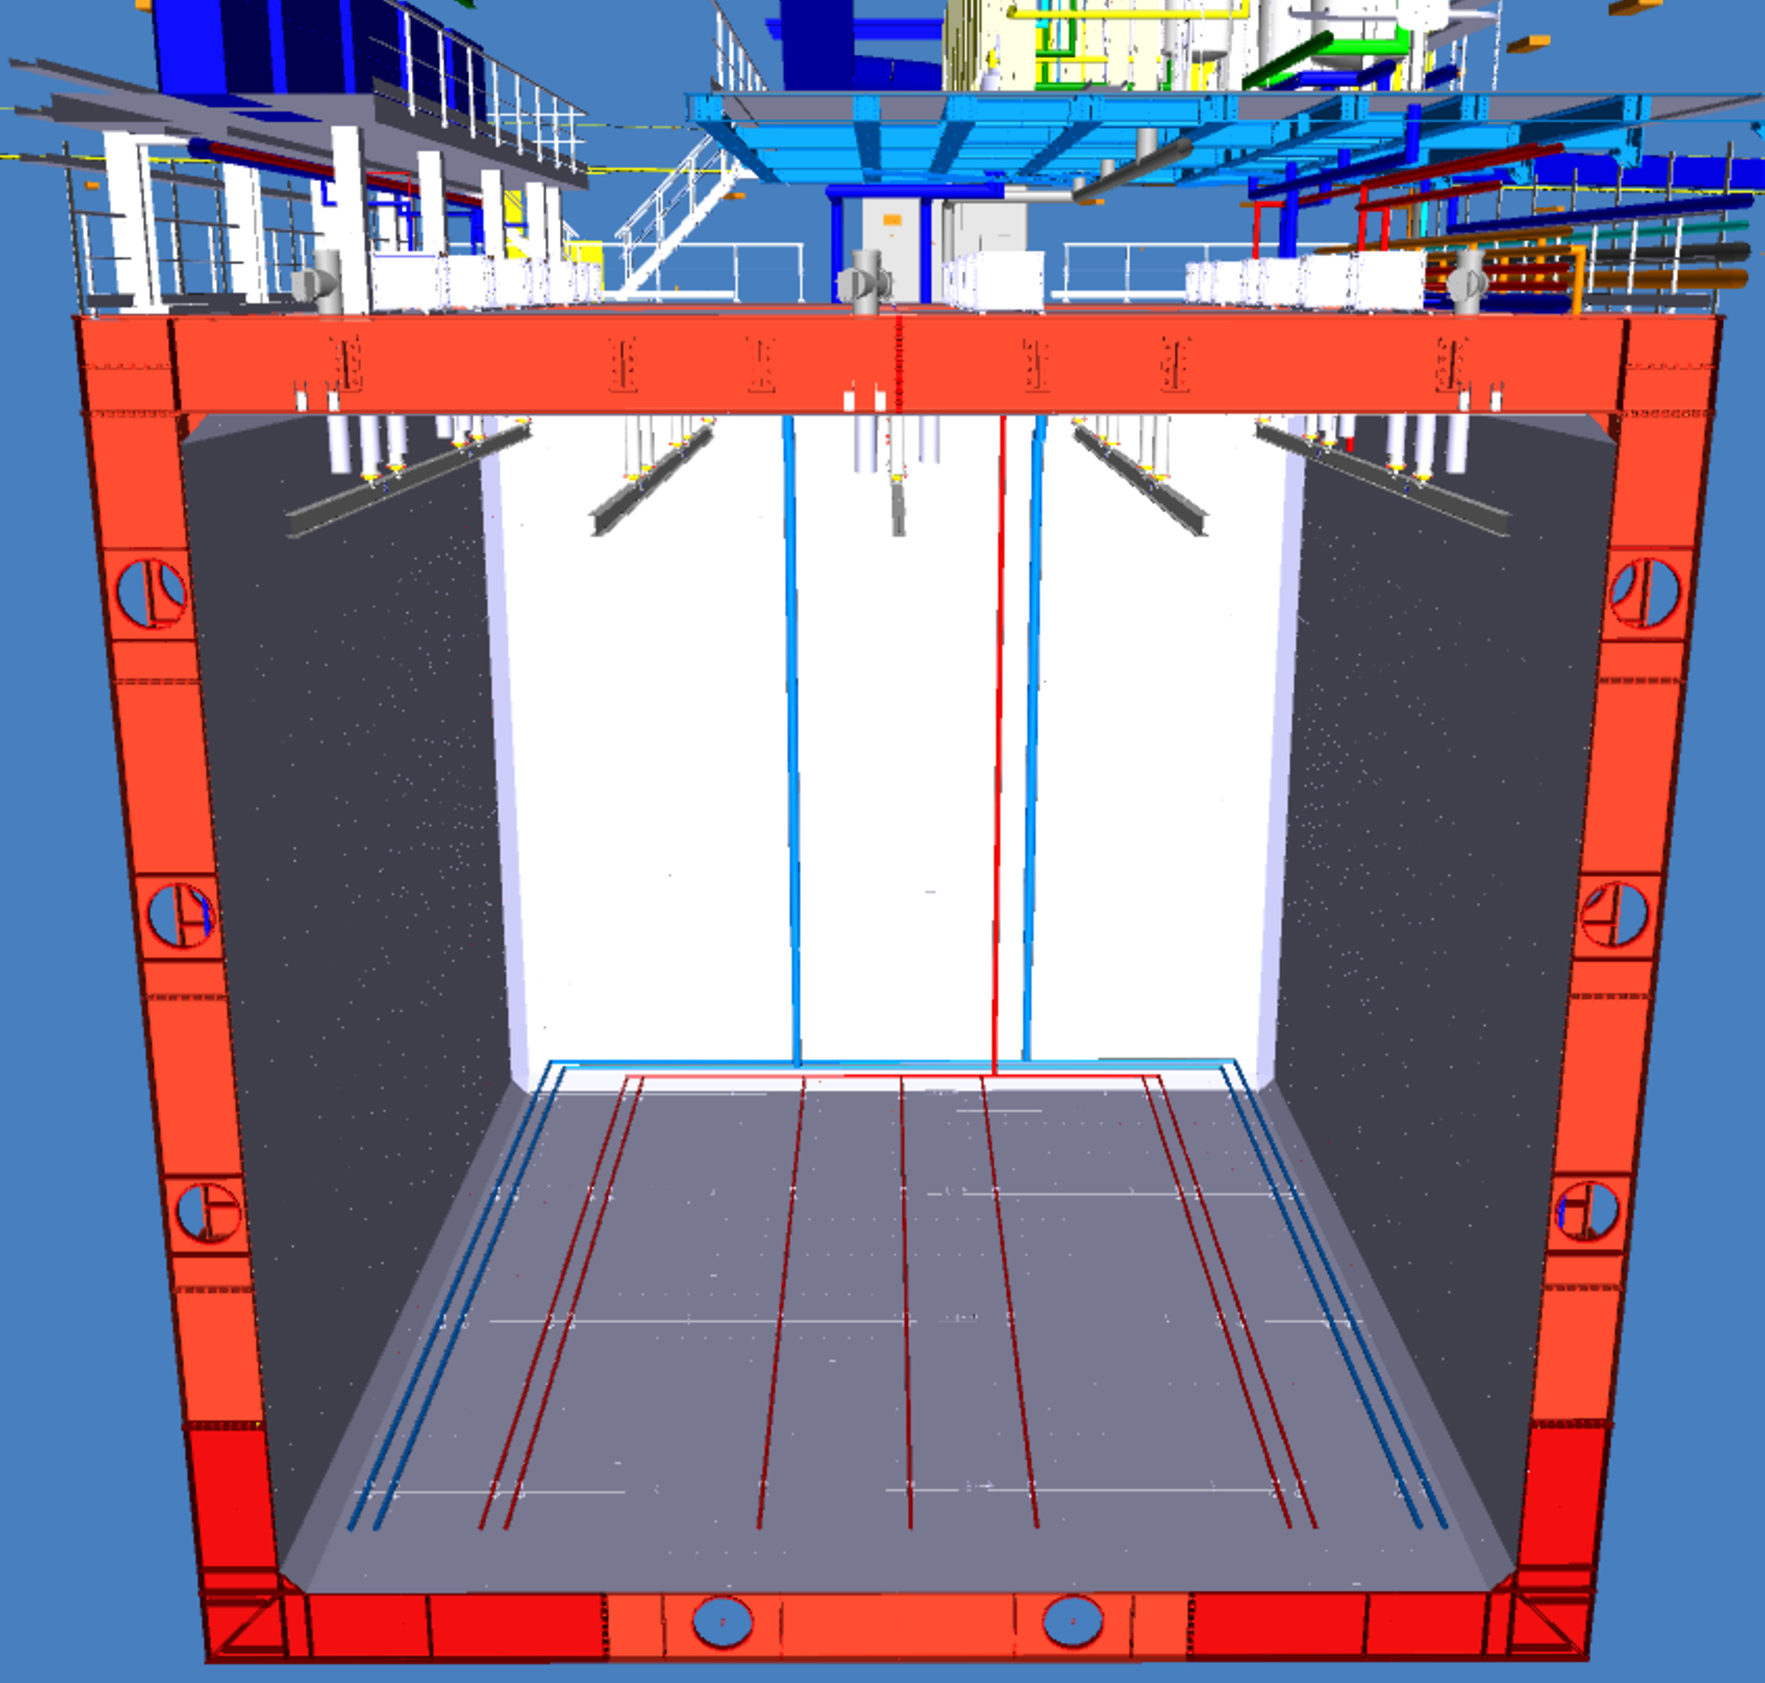
\includegraphics[width=.98\textwidth]{graphics/Internal-Piping-3D.pdf}
\end{dunefigure}

%\begin{dunefigure}[Drawing of the cryogenic %piping inside the cryostat %]{fig:internal-cryo-drawing}
%  {Drawing of the internal cryogenics.}
%\includegraphics[angle=90,width=.98\textwidth]{%graphics/Internal-pipes-HQ.pdf}
%\includegraphics[angle=90,height=.98\textheight%]{graphics/Internal-pipes-HQ.pdf}
%\end{dunefigure}
%\fixme{Please reduce size of Internal-pipes-HQ.pdf}


Other infrastructure inside the cryostat includes the cryostat false floor, the UV filtered lighting, and the battery operated scissor lifts. The false floor is not yet designed as the requirements are not yet fully defined. The false floor must support the load of the scissor lift used to work on the electronic cabling at the cryostat roof inside. It has to be laid out so that the panels can be removed in sections just prior to the equipment installation. The space between the lowest point of the APA modules and the floor is too small to allow the flooring to be removed after the APA is in place. However floor panels in front of the APA need to allow the scissor lift to get close enough to the APA to work comfortably at the top. Careful layout will be needed. 

The cryostat lighting is expected to be a fairly simple based on UV filtered LED lamps. Options for the lighting will be developed during the Ash River testing. Floor mounted lights with task lighting will be investigated. If needed lighting can also be mounted to the DSS and removed as the detector is installed.

The scissor lift is a commercially available battery operated scissor lift with 12 \si{m} reach. Tests will be performed at Ash River to verify the stability of the lift at the 12 \si{m} height. If it is determined that the lift is suitable then the main remaining issue to resolve is the process to install and remove it from the cryostat. The commercially available scissor lifts are too wide to fit through the TCO near the floor where the center post protrudes above floor level. Custom lifting equipment will be needed to insert the lifts into the cryostat. At the end of the installation process it may be necessary to dismantle the last lift to remove it.

% clear the figure buffer before starting the next section
\clearpage

%%%%%%%%%%%%%%%%%%%%%%%%%%%%
\subsection{Cleanroom Infrastructure}
\label{sec:fdsp-tc-infr-comm}

\begin{dunefigure}[Installation Cleanroom layout]{fig:cleanroom-layout}
  {Two views of the installation cleanroom. The walls are semi-transparent so the equipent inside can be seen. The first view from the West looking East shows the materials airlock (orange outline) and changing room (yellow outline). The second image looking North shows the outline of the cleanroom in green where the cryostat is on the right and the airlocks on the right.}
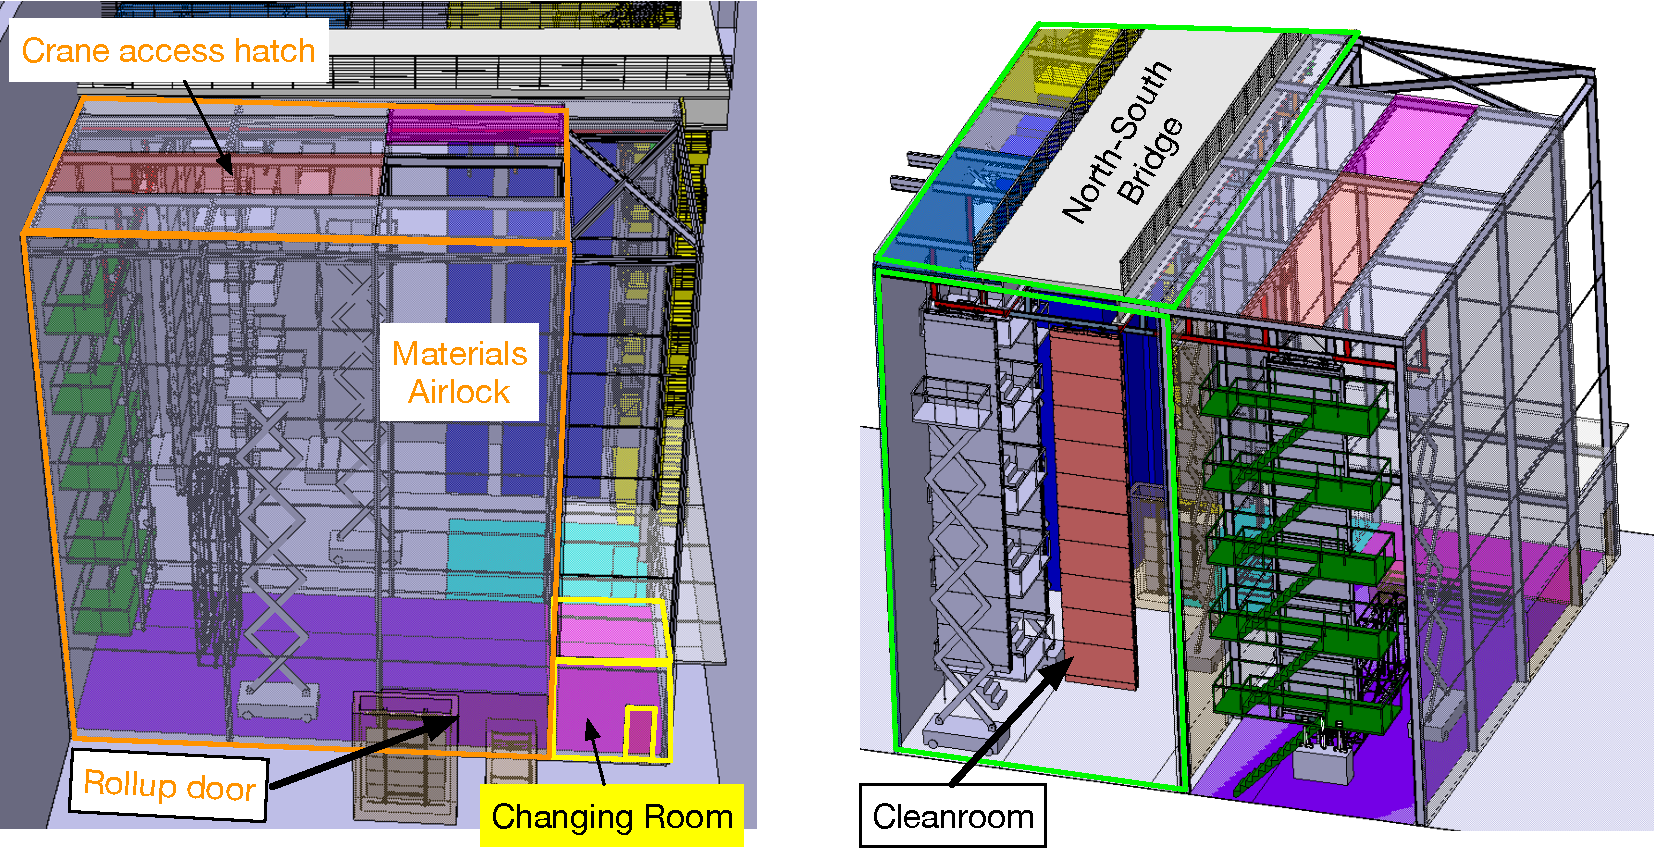
\includegraphics[width=1.0\textwidth]{cleanroom-layout}
\end{dunefigure}

The assembly of the detector sub-components into the 12 \si{m} tall full modules must be done underground directly outside then cryostat. The 12 \si{m} long assemblies are too large and fragile to be brought down the shaft and the only place with enough vertical space to assemble them is in front of the cryostat. The infrastructure work is done by a combination of contractors and the lead worker and rigger teams that will be asisiting in detector assembly. As the cleanliness requirement for all work on the components inside the detector is that all work must be done in an ISO-8 cleanroom a very large cleanroom must be built outside the cryostat that contains all the necessary infrastructure to assemble the detector TPC elements. An image of the conceptual design of the installation cleanroom is shown in Figure \ref{fig:cleanroom-layout}. The left figure is an end view of the cleanroom showing primarily the materials airlock and the changing room. The plan is to bring all the detector elements into the cleanroom through large roll--up doors in the side wall of the airlock. The materials will be moved using using  a battery operated forklift and electric pallet jacks. The airlock is planned to be  13 \si{m} wide 10 \si{m} deep and 17 \si{m} tall. This is sufficiently large to hold the APA assembly tower described below and still have space to move the large objects inside it. An access hatch is planned in the roof which allows the cavern bridge crane to be used in the central area of the airlock. The crane is needed to manipulate the APA modules in the airlock as the plan is to assemble the double high APA pairs here. Also shown on the right of the figure is the changing room for the cleanroom. The changing room is 3 \si{m} wide and 10 \si{m} deep. The dimensions were chosen to allow 20-30 people to gown up for the cleanroom in a reasonable time. The requirements for an ISO-8 cleanroom are a cleanroom lab coat, clean shoes, and hair/beard net. This will be augment with a clean hard hat and gloves for safety reasons. 

The outline of the cleanroom proper is shown on the right in Figure \ref{fig:cleanroom-layout}. The cleanroom dimensions are 16 \si{m} wide 10 \si{m} deep and 17 \si{m} tall. The cleanroom is primarily under the North-South bridge and in the 3.4m space between the bridge and the cryostat. The operations that must be performed in the cleanroom are the cabling of the APA, the cold testing of the APA and the assembly of the cathode-Field cage modules. The tower for the APA cabling, the cold boxes for testing, and the switchyard for moving the 12m tall objects will be described below. All areas of the airlock and cleanroom will be outfitted with UV filtered lights. In addition to the cleanroom shown the inside of the cryostat will also be effectively as cleanroom.  By filtering the air and forcing it  into the cryostat a the East end the clean air will flow through the cryostat and out through the cleanroom and airlock. This will keep the inside of the cryostat also at least at ISO-8. The construction process for the cleanroom is still in a conceptual level and what is shown is a steel frame structure where panels can be mounted. As the size is substantial and the occupancy significant it is expected that it will be outfitted with electrical outlets, UV fileterd lighting and fire protection. 

\fixme{need to check all dimensions and update the figure}

\begin{dunefigure}[APA assembly tower]{fig:apa-assemble-frame}
  {Image of the \dword{apa} assembly tower with the \dword{apa} assembly frame attached. The transport rails at the top of the figure are used to move the assembled \dword{apa} into the cleanroom. The work decks allow access to the \dword{apa} from multiple levels. }
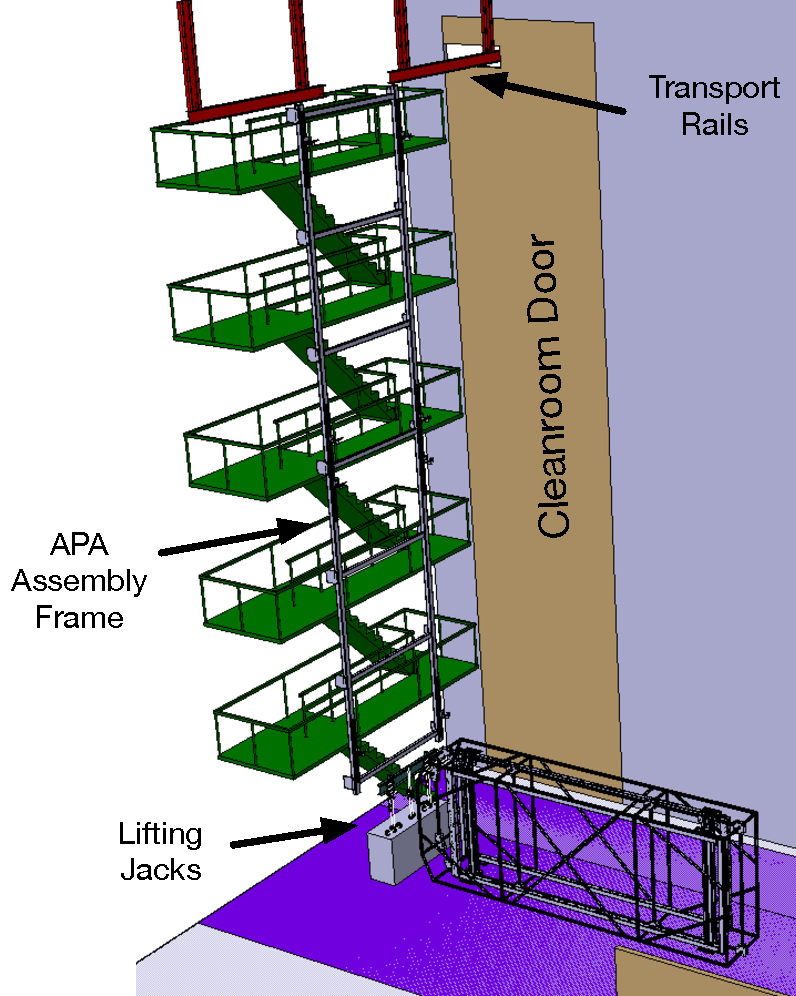
\includegraphics[width=.5\textwidth]{apa-assemble-frame}
\end{dunefigure}
\fixme{need to update the figure}

The APA assembly tower is a 6 story tall stair tower used to assemble the individual APA modules into the final 12 \si{m} tall pair. 
The tower is designed to so that the stair landings will allow access to the sides and top of the APA as required for the assembly. 
The APA assembly tower also provides the support for the the APA assembly fixture provided by the APA consortia. 
The APA assembly fixture is the tooling needed to hold the upper and lower APA during assembly and to bring the two modules together so they can be connected. 
An image of the APA assembly tower is shown in Figure \ref{fig:apa-assemble-frame}. 
In this figure the APA assembly frame is shown mounted on the assembly tower and an APA transport box is on the airlock floor in front of the tower. 
At the top of the APA assembly tower is a set of I-Beam rails used to move the APA pair into the cleanroom through a sliding door shown in brown. 
The final trolleys will be used from this step forward. 
Care will be taken in the APA assembly steps to only remove a minimal amount of the dust protection from the APA at this step in assembly as the manipulations of the APA will need to be performed using the cavern bridge crane which will require an opening in the roof. 
Once the APA are assembled together the bridge crane is no longer needed and the roof opening is closed and the air circulated until the required purity is met. The tower shown in Figure \ref{fig:apa-assemble-frame} has the landings which will meet the safety codes but the outer steel frame to support the landings has not yet been designed.


\begin{dunefigure}[APA cabling tower]{fig:apa-cable-tower}
  {Image of the \dword{apa} cabling tower. The two reels of cable for the electronics are shown. The work decks allow access to the \dword{apa} from multiple levels. }
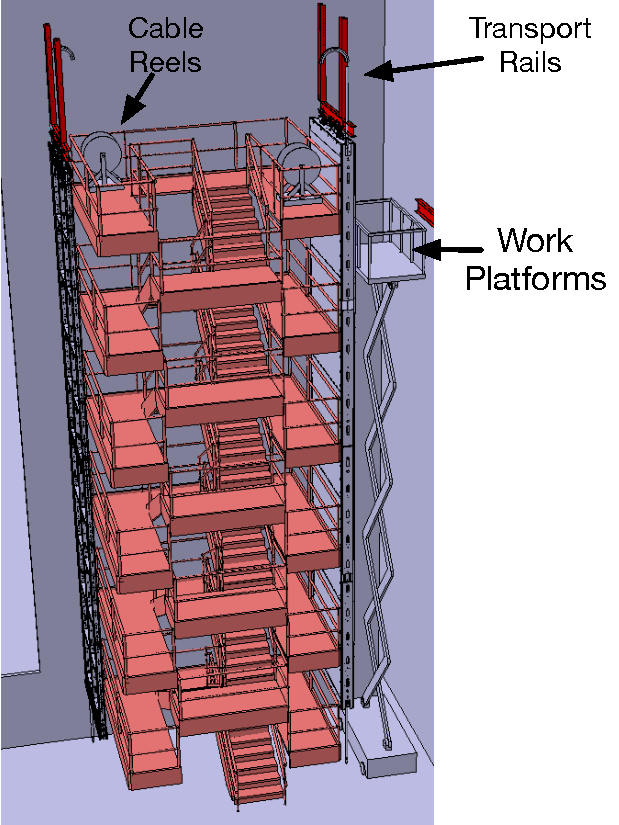
\includegraphics[width=.5\textwidth]{apa-cable-tower}
\end{dunefigure}

Inside the cleanroom is another stair tower used for the cabling and initial test of the cold electronics. Based on the time required for the cabling and testing of the electronics in ProtoDUNE it is expected that one will need two workstations. The APA cabling tower is shown in Figure \ref{fig:apa-cable-tower}. The APA cabling tower is a stair tower similar to the APA assembly tower where access is provided to the sides of the APA at numerous levels and a dedicated lift provides access on the outer face. The cable is brought up to the top of the platform in spools using the switchyard described below. The APA are move next to the stair tower work faces also using the switchyard.  Sufficient space is needed at the top levels to allow people to work on the cabling and to test the electronics. The size and the layout of the top level of the tower will be optimized based on the input from the prototyping tests to be done at Ash River. 

\begin{dunefigure}[Cleanroom material transport system]{fig:cleanroom-switchyard}
  {The switchyard inside the cleanroom and airlock is shown. In this figure the beams of the switchyard are shown highlited in red. Fixed beams running East-West are used to move the APA and CPA to dedicated work location while a bridge crane running North-South is used to transport the units between the different fixed beams. }
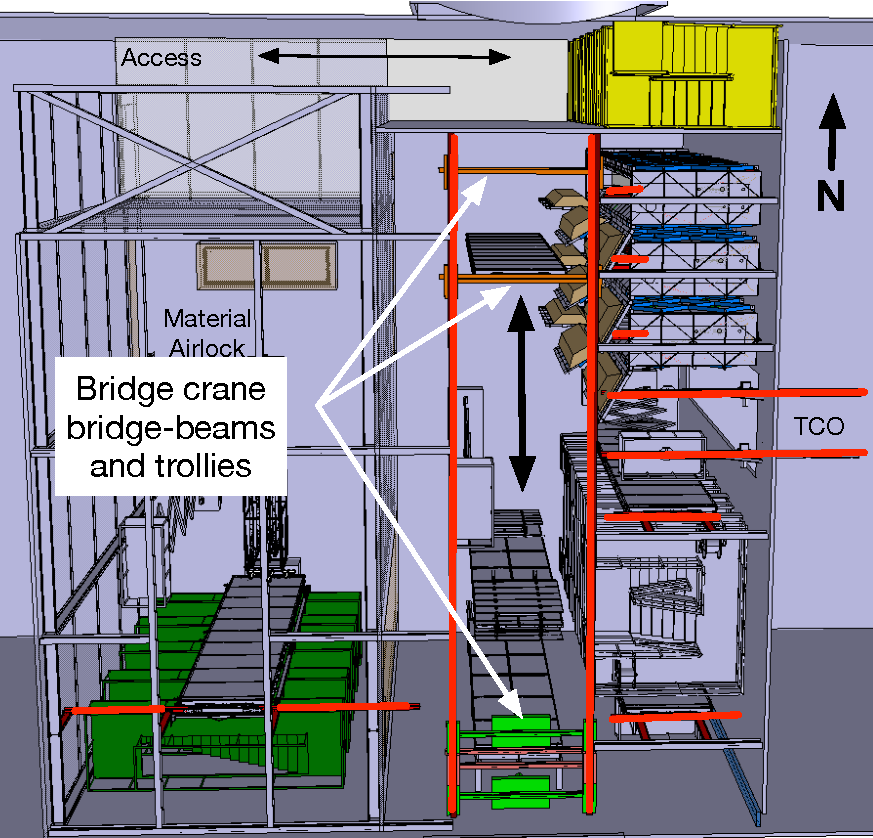
\includegraphics[width=.75\textwidth]{cleanroom-switchyard}
\end{dunefigure}

Once the APA pair or the CPA panels are assembled the units will be moved around the cleanroom and airlock using a dedicated rail based switchyard (I-beam and trolley). An image of the switchyard is shown in Figure \ref{fig:cleanroom-switchyard}. In the center of the figure is the bride crane which travels North-South. Several bridge beams driven by electric trolleys will move on the runway beams of the crane.  By aligning the bridge beams with a set of fixed beams supported from the cleanroom roof the APA and CPA can be transferred from the fixed beams to the bridge crane and then moved to different locations in the cleanroom. In Figure \ref{fig:cleanroom-switchyard} a single fixed beam in front of the APA assembly tower in airlock and seven locations on the right where equipment's can be moved for various steps in the assembly and testing. The work stations are the two faces of the APA cabling tower, the 2 beams through the TCO used to move the finished detector into the cryostat and the 3 I-Beams used to move the APA into the cold boxes in the North--East corner of the cleanroom. An additional fixed beam will need to be added over the cabling tower to allow the cable reals to be hoisted to the top. 

%%%%%%%%%%%%%%%%%%%%%%%%%%%%
\subsection{Cryogenics and Cold-Boxes}
\label{sec:fdsp-tc-infr-cryo}
After the APA pairs are fully assembled and cabled they are thermally cycled before being installed in the cryostat. To do this three tall but narrow cryostat are needed that can be cooled as close to LAr temperature as reasonably possible. These cryostats are referred to as cold--boxes and require a dedicated cryogenics system. 



The cold--boxes used to thermally cycle the assembled APA pairs prior to installation in the cryostat are shown in Figure \ref{fig:install-coldbox}. 
In order to test APAs at the rate needed to keep up with the installation plan three cold--boxes are needed inside the cleanroom. 
Each cold--box has external dimensions of 14.0 \si{m} by 3.2 \si{m} by 1.3 \si{m} (H $\times$ L $\times$ W). 
Three layers of 100 \si{mm} thick foam insulation are used for the thermal isolation. 
This gives an internal dimensions of 13.4 \si{m} x 2.6 \si{m} x 0.7 \si{m} (H $\times$ L $\times$ W). 
Inside each cold--box a rail section similar to what is used in the TCO and other fixed rails in the cleanroom will be mounted.
This will allow the APA to be pushed into the coldboxes using the cleanroom switchyard and trolleys. 
A support base will be needed under the cold--boxes to adjust the height in order to mate with the cleanroom switchyard.
The cold--boxes will have an electronics feedthru similar to what is used on the top of the DUNE cryostat, except that short cables will be used to run from the WEC to a patch panel inside the cold-box.
This will allow the cable on the APA to be connected directly to the test readout without having to un-do any cabling. 
Each cold--box will be designed similar to the successful ProtoDUNE-SP cold--box. 
The outer shell is constructed of stainless plate which has reinforcing ribs welded on. 
The biggest difference between the DUNE cold-boxes and the ProtoDUNE-SP cold--box other than doubling the height is that a hinged door is planned for the DUNE cold-boxes. 
In Proto-DUNE significant effort was needed to unbolt and lift off the door of the coldbox. 
In DUNE the cleanroom does not have full crane coverage so doors that can be opened and closed using a scissor lift are required.
Initial estimates are that the DUNE cold--boxes will need about 11 \si{T} of stainless steel. 
They will need to be assembled in place as the finished boxes are too big to fit down the Ross Shaft. 
The cold-box base will need be placed on Hilman rollers so the boxes can be moved under the bridge at the end of installation allowing for the installation of the cryogenic circulation pumps.
 





\begin{dunefigure}[Installation Cold--box]{fig:install-coldbox}
  {Cold--boxes used to thermally cycle the fully assembled APA pairs. }
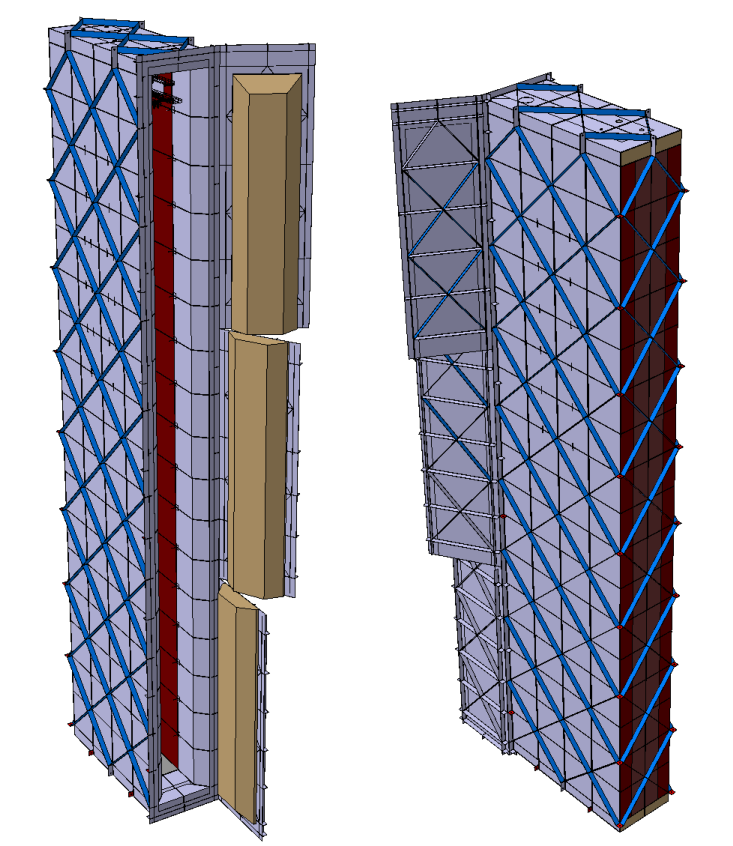
\includegraphics[width=.5\textwidth]{graphics/install-coldbox.pdf}
\end{dunefigure}

%DAVID added cryo cold box%%
\subsubsection{Cryogenics supporting the Cold--Boxes}
%{Cold Boxes Cryogenics}
\label{sec:fdsp-tc-cryocoldbox}

%The cryogenics supporting the \coldbox{}es underground must ensure reliable and safe operation of the system used to test the \dwords{apa} that will be installed inside the cryostats. The main functional requirements of the system are
The  \coldbox{}es will be used to test the \dword{apa}s underground prior to installation. % in the cryostat. 
The cryogenics supporting the \coldbox{}es  must ensure their reliable and safe operation; to that end, it must
\begin{itemize}
\setlength\itemsep{1mm}
\setlength{\parsep}{1mm}
\setlength{\itemsep}{-5mm}
\item support three \coldbox{}es operating in parallel: %for testing dual \dword{apa}s: 
one in \cooldown mode, two either in steady-state or warm-up modes.
\item allow personnel in the cleanroom during all phases of the purge, \cooldown, operation, and warm-up modes. 
\item test the detector modules at near \dword{lar} temperature.
\item operate 24 hours a day, seven days a week for 10 years.
\item allow remote operations.
\item be located in the vicinity of the \dword{tco}. Space is available on top of the cryogenic mezzanine on the roof of the cryostat.
\end{itemize}

It must operate in the following modes: %fulfill the following modes of operations:

\begin{itemize}
\setlength\itemsep{1mm}
\setlength{\parsep}{1mm}
\setlength{\itemsep}{-5mm}
\item \textbf{purge}: During this mode, air is removed from the system (\coldbox and cryogenic system) and replaced with dry nitrogen. The concentration of moisture is monitored, and when it no longer decreases, the \cooldown can commence.
\item \textbf{\cooldown}: Cold nitrogen is introduced into the system to cool the inside of the \coldbox and the \dword{apa} inside it. %it down and to cool down the detector contained inside the coldbox. 
This should take 24 hours, during which time the temperature decreases from room temperature to about \SI{90}{K}. 
\item \textbf{steady-state operations}: After reaching %the nominal temperature of 
approximately \SI{90}{K}, %the value is maintained for 48 hours, during which 
the detector is turned on and fully tested. % at cold. 
This takes about 48 hours.
\item \textbf{warm-up}: After completing the test, the system is %slowly 
warmed up to room temperature over a period of 24 hours. %This should take 24 hours, during which the temperature goes from approximately \SI{90}{K} to room temperature.
\end{itemize}

\begin{dunetable}
[\Coldbox  cryogenics system parameters] %for specifications]
{lc}
{tab:table-cryo-coldboxes}
{Table of parameters for the \coldbox cryogenics system.}
Parameter & Value 
\\ \toprowrule
Dual \dword{apa} thermal mass &  1,600 kg\\ \colhline
Temperature uniformity & $+60$ K / $-0$ K \\ \colhline
Electronics load & 300 W \\ \colhline
\Coldbox insulation thickness &  0.3 m \\ \colhline
Target \cooldown temperature &  \SI{90}{K} \\ \colhline
Target \cooldown duration &  24 hr \\ \colhline
Target steady-state duration &  48 hr \\ \colhline
Target warm-up duration &  24 hr \\ \colhline
Maximum cooling power  &  \SI{13}{kW}  \\ \colhline 
Maximum liquid nitrogen consumption  &  \SI{300}{l/hr}  \\ \colhline 
\end{dunetable}

The evaporation of liquid nitrogen provides the cooling power for the system. Warm nitrogen and a heater provide the heating power. At peak consumption, the expected maximum heat load is \SI{8.5}{kW}. Assuming a 50\% margin on the refrigeration load, the cryogenics system requires \SI{13}{kW} of net cooling power at peak consumption, which equals about \SI{300}{l/hr} of evaporating liquid nitrogen.

Two layouts are currently under consideration: (1) a closed loop with mechanical refrigeration, in which liquid nitrogen is generated {\it in situ}, circulated, and the spent nitrogen recondensed before being put back into the system; and (2) open loop, in which liquid nitrogen is transported underground by means of portable dewars, circulated, and the spent nitrogen vented away. For the closed loop, we would need a mechanical refrigeration capable of supplying \SI{13}{kW} of cooling. For the open loop, it is possible to use a \SI{2000}{l} dewar, which is commercially available and transportable up and down the Ross Shaft inside the cage. To supply the required amount of nitrogen, four trips per day are needed.

The current versions of the closed loop and open loop systems are presented in Figures~\ref{fig:mechanical-refrigeration} and~\ref{fig:LN2}, respectively. % . The current version of the open loop system is presented in Figure~\ref{fig:LN2}.

\begin{dunefigure}[\Coldbox cryogenics support system based on mechanical refrigeration ]{fig:mechanical-refrigeration}
  {Layout of the cryogenics supporting the \dword{apa} test facility with mechanical refrigeration (closed loop).}
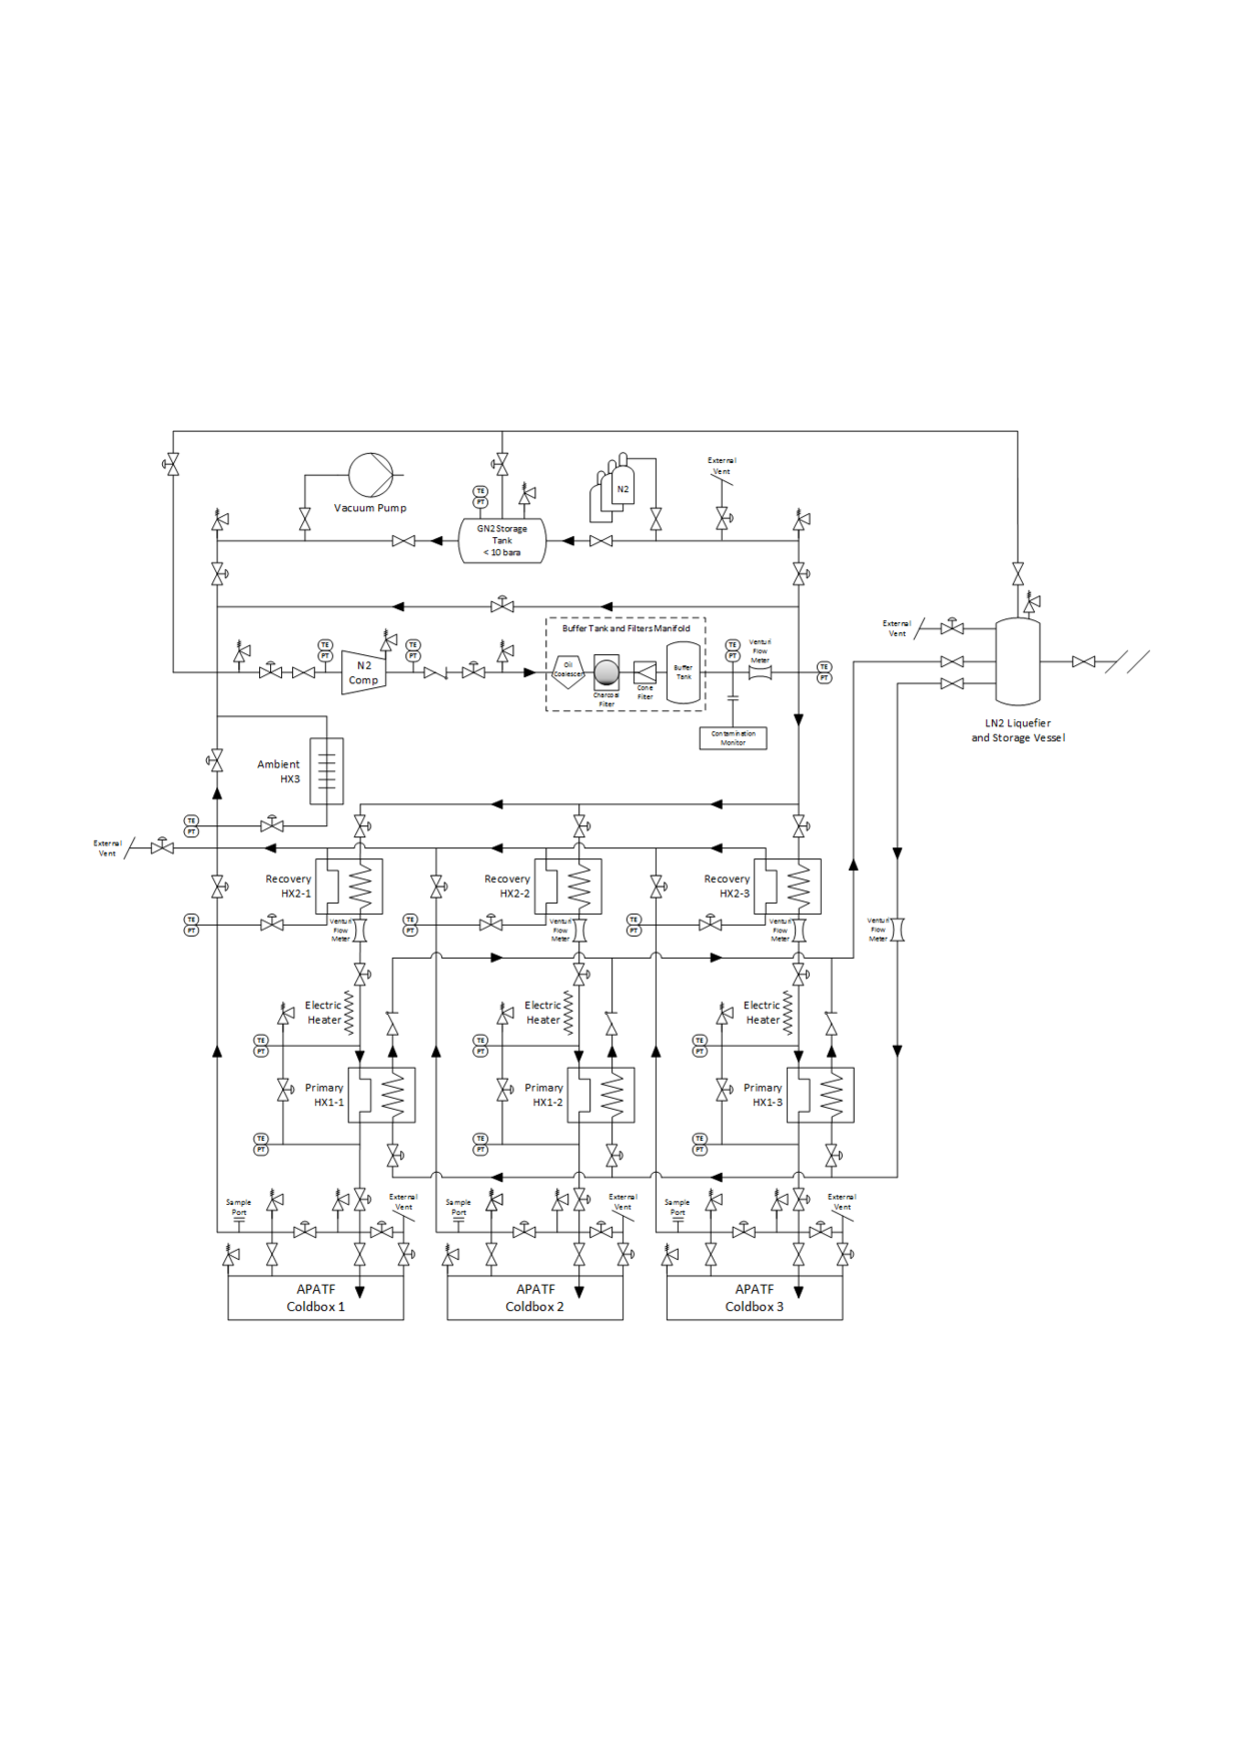
\includegraphics[width=.98\textwidth]{graphics/Cryo-cold-box-mechanical.pdf}
\end{dunefigure}

\begin{dunefigure}[\Coldbox cryogenics support system based on LN2 ]{fig:LN2}
  {Layout of the cryogenics supporting the \dword{apa} test facility with open loop refrigeration (open loop).}
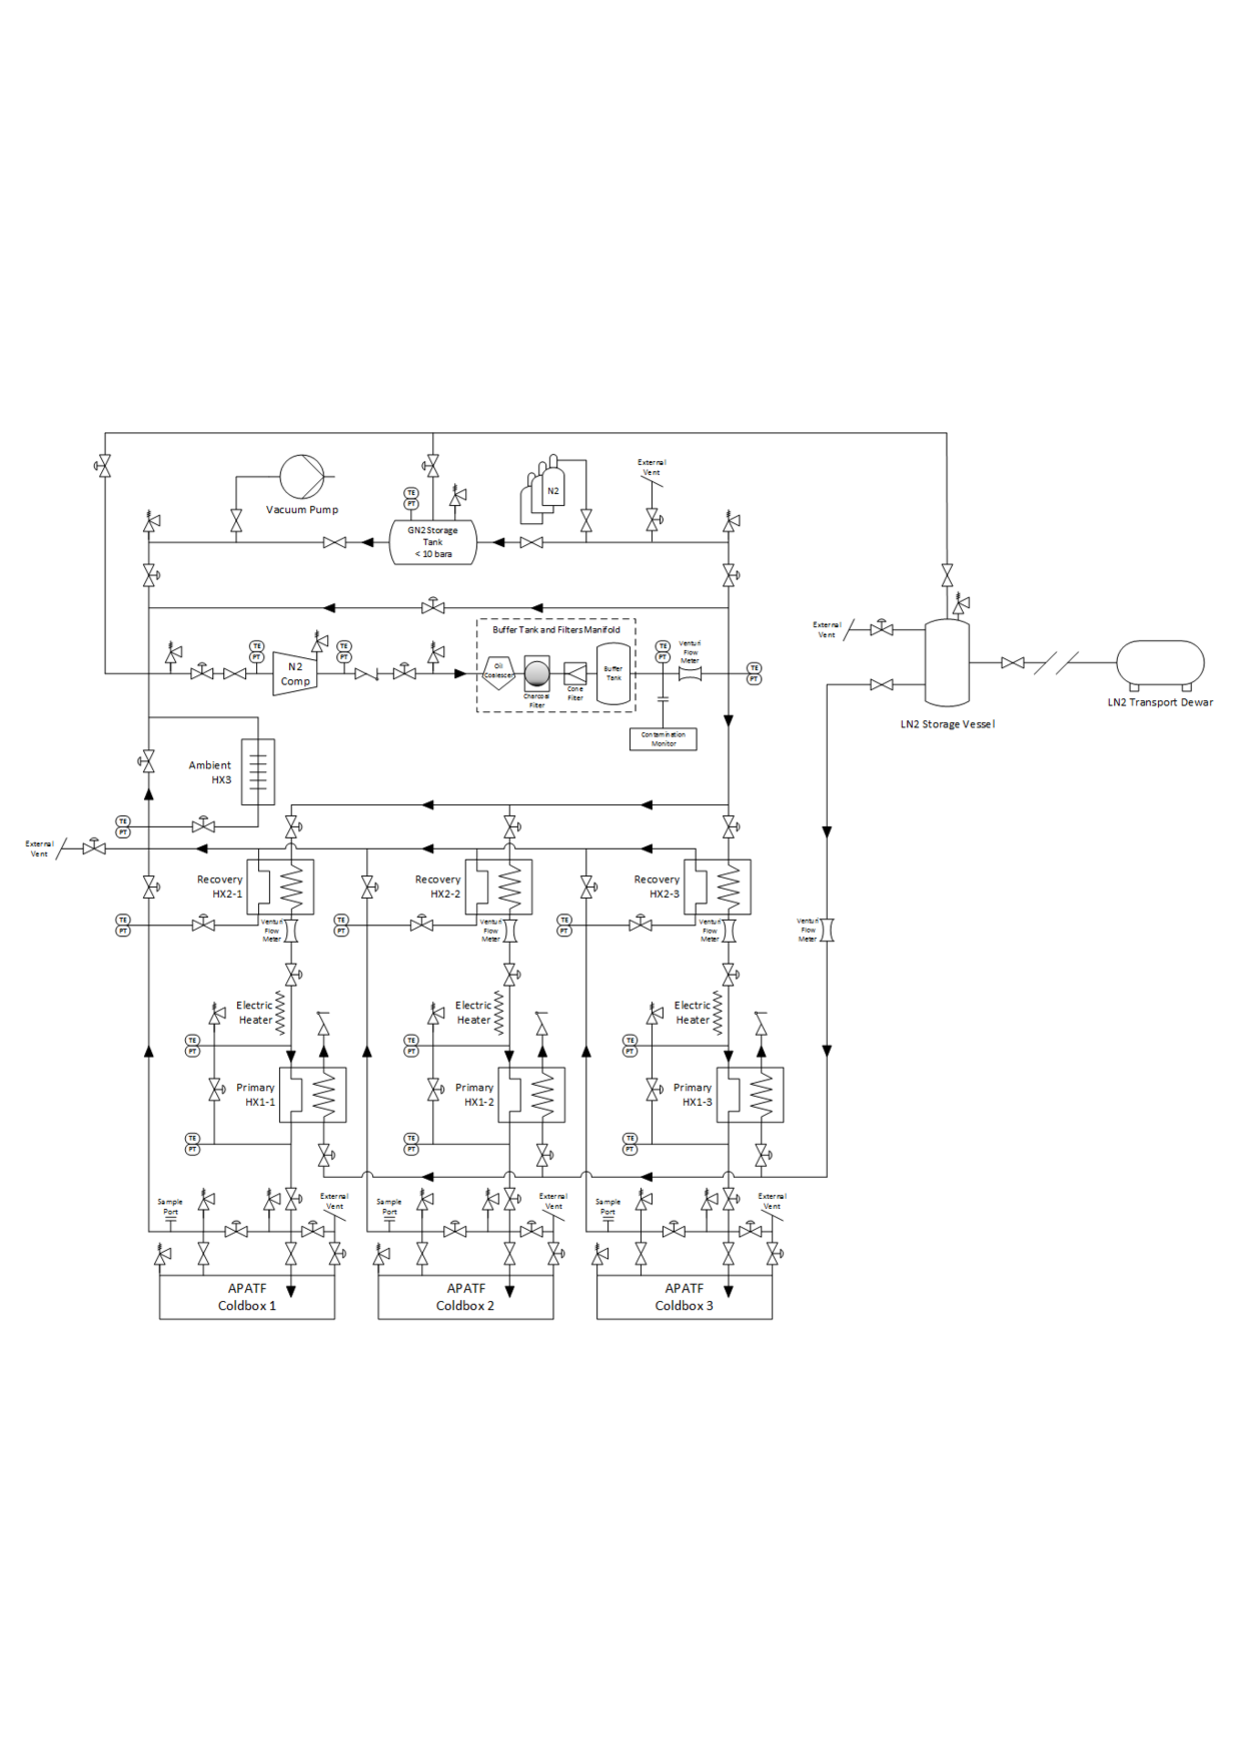
\includegraphics[width=.98\textwidth]{graphics/Cryo-cold-box-LN2.pdf}
\end{dunefigure}



%%%%%%%%%

% clear the figure buffer before starting the next section
\clearpage

%%%%%%%%%%%%%%%%%%%%%%%%%%%%
\subsection{Prototyping and Testing (QA/QC)}
\label{sec:fdsp-tc-infr-qaqc}
This is the critical phase where all of the new installation equipment is installed underground.  While the majority of these installation procedures have already been tested during the Trial Assembly at Ash River everything must be properly approved. the main APA and CPA towers will already be structurally approved but load tests will have to be performed on all the lifting fixtures, shuttle beams, cranes tower connections and cold box connections. 

This is also the time period that the cold boxes and cryogenic system will be tested, this time period will certainly have numerous days that access to the cleanroom may be restricted during system checks.


%%%%%%%%%%%%%%%%%%%%%%%%%%%%
\subsection{Safety}
\label{sec:fdsp-tc-infr-safety}
This is the phase of construction of Detector 1 that we have larger teams from the consortia, SDSD  and contractors underground at the same time LBNF is working completing the cold structure on Detector 1 and beginning the warm structure on detector 2.. Our shift schedule now switches to 2 shifts/day since we are confined to a maximum of 140 FTE underground at any given time.  Daily work meetings and safety coordination lead by the shift supervisor at the start of each shift to coordinate work activities, review hazards/mitigation and installation procedures are critical for a safe work environment. More details can be found in section 1.4.4 under the Installation ESH section. 

The UIT (Underground Installation Team) will be extremely busy during this period. The crew sizes are increasing so training of new employees and consortia, new equipment is being installed and tested. Proper documentation including structural calculations, assembly drawings, load tests, hazard analyses and procedures will all have to be reviewed and approved before Operational Readiness is approved. This all helps prepare for a safe start to the installation underground. 

The cold box and cryogenic system is one of the few things in the installation process that will not be fully tested during any of the trial assembly work. While the design of the boxes are very similar to the what was done at CERN for ProtoDUNE the major difference is the system requirement that it is safe for workers to be in the cleanroom during the cool down phase. Procedures for operation of the cold box have not been defined but a requirements document has been written.   

%%%%%%%%%%%%%%%%%%%%%%%%%%%%
\subsection{Costs, Schedule and Risk Analysis}
\label{sec:fdsp-tc-infr-cost}

\fixme{Add costs when available}

{\bf Installation Setup Phase:} This is a more difficult phase to schedule and may be adjusted often with multiple projects going on at once. The CF work is basically completed which reduces the number of FTEs underground allowing us to begin the installation Infrastructure. We begin two 10 hour sifts per day as the work ramps up.  Once the cold cryostat is roughly 6 months into their installation schedule floor space becomes available in the North Cavern. The cold box construction needs to be started ASAP since the welding process takes $\sim6$ months. In parallel to this the work the shop area, the bridge between the North and South sides of the cavern can be constructed. Once the bridge is completed work on the assembly crane, APA Cabling Tower, APA Assembly Tower and CPA assembly station. 
    
Potentially the installation of the detector support system will happen during the final stages of the cryostat cold structure since they require full height scaffolding to do all the welding on the top of the cryostat. This was how the ProtoDUNE DSS was installed. The details have not been worked out yet with the contractor so work may be done in stages. It requires a crew on the top of the cryostat installing the DSS support feedthrus from the top of the cryostat as shown in figure 1.25. 
    
A detailed schedule of the installation infrastructure time period is shown in Figure~\ref{fig:Installation_Infrastructure_Schedule}
    
\begin{dunefigure}[Schedule for the infrastructure installation]
{fig:Installation_Infrastructure_Schedule}
    {Installation Infrastructure Schedule}
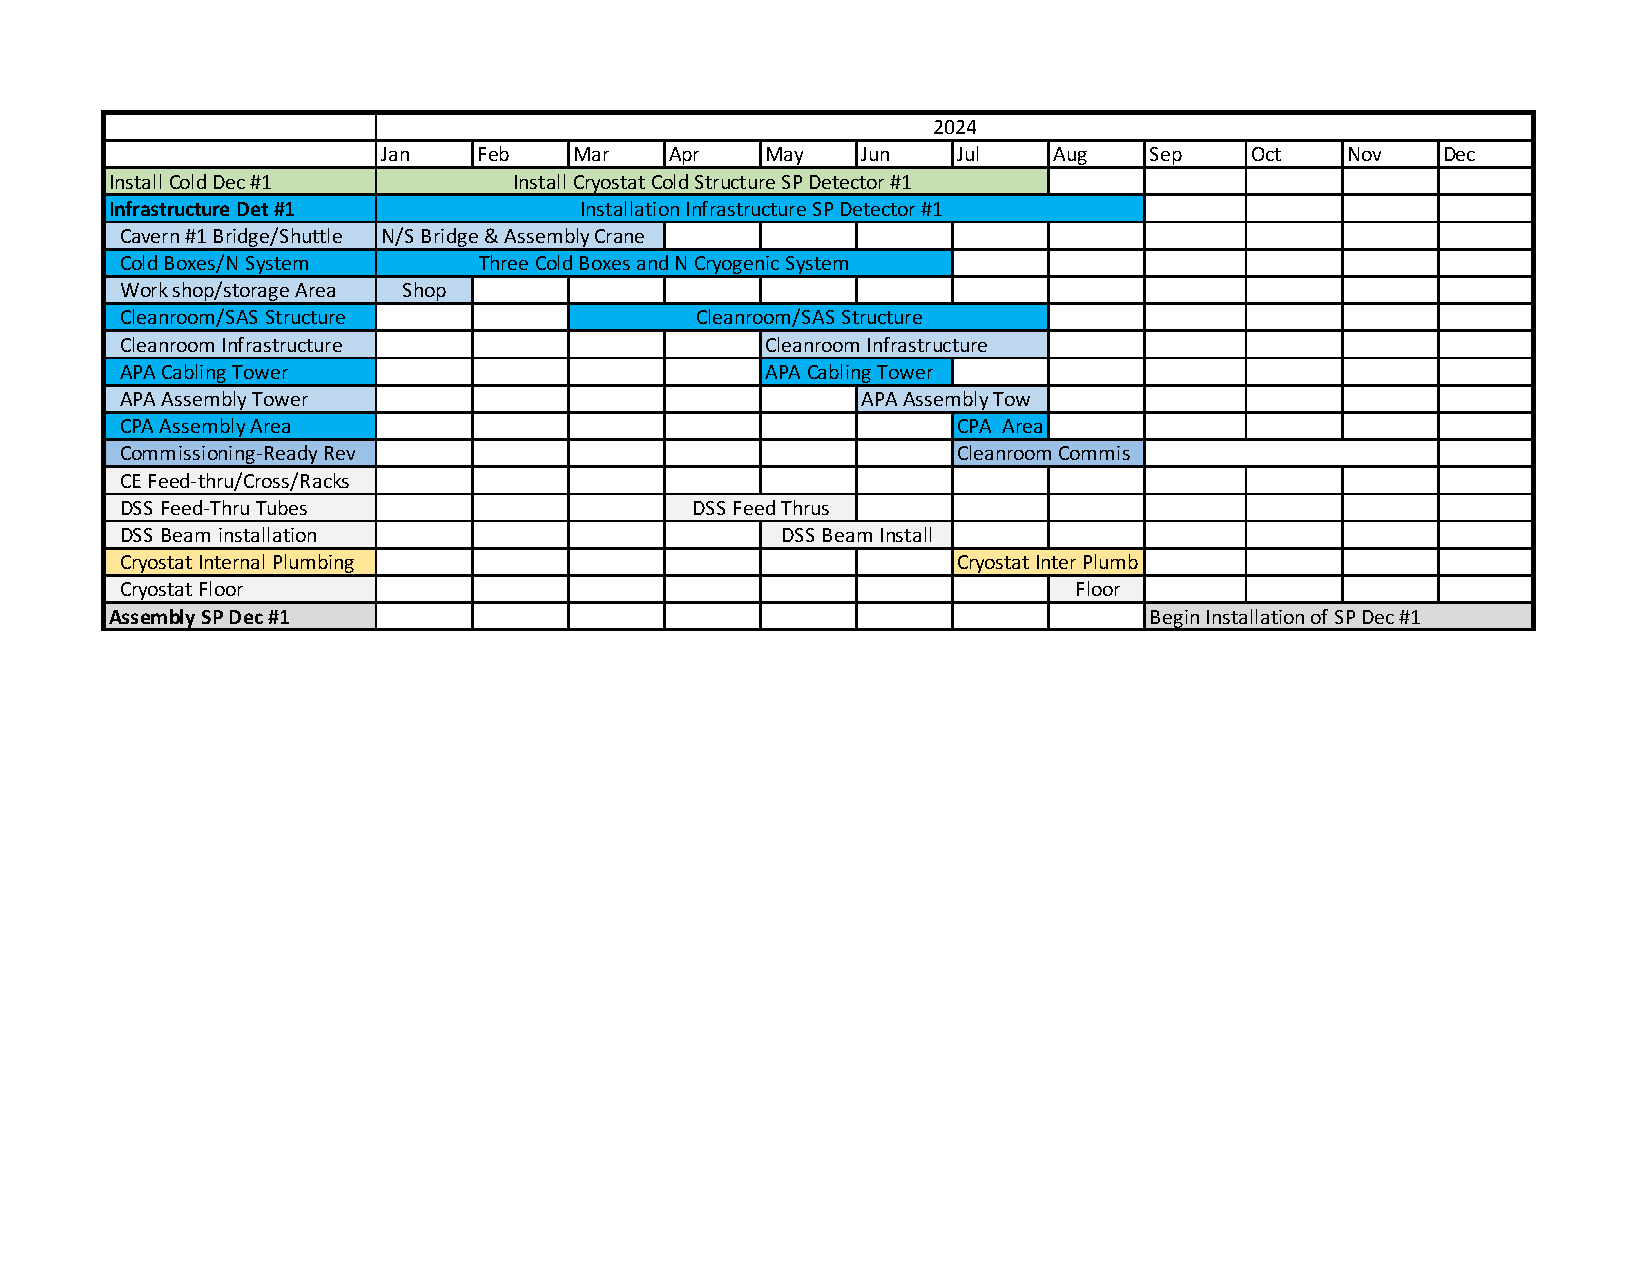
\includegraphics[width=0.98\textwidth]
{Installation_Infrastructure_Schedule} 
\end{dunefigure}

\fixme{use templates from cost-risk-sched.tex file. Anne}

% clear the figure buffer before starting the next section
\clearpage
